% Options for packages loaded elsewhere
\PassOptionsToPackage{unicode}{hyperref}
\PassOptionsToPackage{hyphens}{url}
%
\documentclass[
]{article}
\usepackage{amsmath,amssymb}
\usepackage{iftex}
\ifPDFTeX
  \usepackage[T1]{fontenc}
  \usepackage[utf8]{inputenc}
  \usepackage{textcomp} % provide euro and other symbols
\else % if luatex or xetex
  \usepackage{unicode-math} % this also loads fontspec
  \defaultfontfeatures{Scale=MatchLowercase}
  \defaultfontfeatures[\rmfamily]{Ligatures=TeX,Scale=1}
\fi
\usepackage{lmodern}
\ifPDFTeX\else
  % xetex/luatex font selection
\fi
% Use upquote if available, for straight quotes in verbatim environments
\IfFileExists{upquote.sty}{\usepackage{upquote}}{}
\IfFileExists{microtype.sty}{% use microtype if available
  \usepackage[]{microtype}
  \UseMicrotypeSet[protrusion]{basicmath} % disable protrusion for tt fonts
}{}
\makeatletter
\@ifundefined{KOMAClassName}{% if non-KOMA class
  \IfFileExists{parskip.sty}{%
    \usepackage{parskip}
  }{% else
    \setlength{\parindent}{0pt}
    \setlength{\parskip}{6pt plus 2pt minus 1pt}}
}{% if KOMA class
  \KOMAoptions{parskip=half}}
\makeatother
\usepackage{xcolor}
\usepackage[margin=1in]{geometry}
\usepackage{color}
\usepackage{fancyvrb}
\newcommand{\VerbBar}{|}
\newcommand{\VERB}{\Verb[commandchars=\\\{\}]}
\DefineVerbatimEnvironment{Highlighting}{Verbatim}{commandchars=\\\{\}}
% Add ',fontsize=\small' for more characters per line
\usepackage{framed}
\definecolor{shadecolor}{RGB}{248,248,248}
\newenvironment{Shaded}{\begin{snugshade}}{\end{snugshade}}
\newcommand{\AlertTok}[1]{\textcolor[rgb]{0.94,0.16,0.16}{#1}}
\newcommand{\AnnotationTok}[1]{\textcolor[rgb]{0.56,0.35,0.01}{\textbf{\textit{#1}}}}
\newcommand{\AttributeTok}[1]{\textcolor[rgb]{0.13,0.29,0.53}{#1}}
\newcommand{\BaseNTok}[1]{\textcolor[rgb]{0.00,0.00,0.81}{#1}}
\newcommand{\BuiltInTok}[1]{#1}
\newcommand{\CharTok}[1]{\textcolor[rgb]{0.31,0.60,0.02}{#1}}
\newcommand{\CommentTok}[1]{\textcolor[rgb]{0.56,0.35,0.01}{\textit{#1}}}
\newcommand{\CommentVarTok}[1]{\textcolor[rgb]{0.56,0.35,0.01}{\textbf{\textit{#1}}}}
\newcommand{\ConstantTok}[1]{\textcolor[rgb]{0.56,0.35,0.01}{#1}}
\newcommand{\ControlFlowTok}[1]{\textcolor[rgb]{0.13,0.29,0.53}{\textbf{#1}}}
\newcommand{\DataTypeTok}[1]{\textcolor[rgb]{0.13,0.29,0.53}{#1}}
\newcommand{\DecValTok}[1]{\textcolor[rgb]{0.00,0.00,0.81}{#1}}
\newcommand{\DocumentationTok}[1]{\textcolor[rgb]{0.56,0.35,0.01}{\textbf{\textit{#1}}}}
\newcommand{\ErrorTok}[1]{\textcolor[rgb]{0.64,0.00,0.00}{\textbf{#1}}}
\newcommand{\ExtensionTok}[1]{#1}
\newcommand{\FloatTok}[1]{\textcolor[rgb]{0.00,0.00,0.81}{#1}}
\newcommand{\FunctionTok}[1]{\textcolor[rgb]{0.13,0.29,0.53}{\textbf{#1}}}
\newcommand{\ImportTok}[1]{#1}
\newcommand{\InformationTok}[1]{\textcolor[rgb]{0.56,0.35,0.01}{\textbf{\textit{#1}}}}
\newcommand{\KeywordTok}[1]{\textcolor[rgb]{0.13,0.29,0.53}{\textbf{#1}}}
\newcommand{\NormalTok}[1]{#1}
\newcommand{\OperatorTok}[1]{\textcolor[rgb]{0.81,0.36,0.00}{\textbf{#1}}}
\newcommand{\OtherTok}[1]{\textcolor[rgb]{0.56,0.35,0.01}{#1}}
\newcommand{\PreprocessorTok}[1]{\textcolor[rgb]{0.56,0.35,0.01}{\textit{#1}}}
\newcommand{\RegionMarkerTok}[1]{#1}
\newcommand{\SpecialCharTok}[1]{\textcolor[rgb]{0.81,0.36,0.00}{\textbf{#1}}}
\newcommand{\SpecialStringTok}[1]{\textcolor[rgb]{0.31,0.60,0.02}{#1}}
\newcommand{\StringTok}[1]{\textcolor[rgb]{0.31,0.60,0.02}{#1}}
\newcommand{\VariableTok}[1]{\textcolor[rgb]{0.00,0.00,0.00}{#1}}
\newcommand{\VerbatimStringTok}[1]{\textcolor[rgb]{0.31,0.60,0.02}{#1}}
\newcommand{\WarningTok}[1]{\textcolor[rgb]{0.56,0.35,0.01}{\textbf{\textit{#1}}}}
\usepackage{graphicx}
\makeatletter
\def\maxwidth{\ifdim\Gin@nat@width>\linewidth\linewidth\else\Gin@nat@width\fi}
\def\maxheight{\ifdim\Gin@nat@height>\textheight\textheight\else\Gin@nat@height\fi}
\makeatother
% Scale images if necessary, so that they will not overflow the page
% margins by default, and it is still possible to overwrite the defaults
% using explicit options in \includegraphics[width, height, ...]{}
\setkeys{Gin}{width=\maxwidth,height=\maxheight,keepaspectratio}
% Set default figure placement to htbp
\makeatletter
\def\fps@figure{htbp}
\makeatother
\setlength{\emergencystretch}{3em} % prevent overfull lines
\providecommand{\tightlist}{%
  \setlength{\itemsep}{0pt}\setlength{\parskip}{0pt}}
\setcounter{secnumdepth}{-\maxdimen} % remove section numbering
\usepackage{hyperref}
\usepackage{amsmath}
\usepackage{amssymb}
\usepackage{graphicx}
\usepackage{fontspec}
\setmainfont{Cambria}
\setsansfont{Franklin Gothic Demi Cond}
\setmonofont{Courier New}
\usepackage[margin=1in]{geometry}
\usepackage{titlesec}
\titleformat{\section}{\Huge\bfseries\color{black}}{\thesection}{1em}{}
\titleformat{\subsection}{\huge\bfseries\color{black}}{\thesubsection}{1em}{}
\titleformat{\subsubsection}{\LARGE\bfseries\color{black}}{\thesubsubsection}{1em}{}
\usepackage{tocloft}
\renewcommand{\cftsecfont}{\small}
\renewcommand{\cftsubsecfont}{\footnotesize}
\renewcommand{\cftsecpagefont}{\small}
\renewcommand{\cftsubsecpagefont}{\footnotesize}
\renewcommand{\cftsecleader}{\cftdotfill{\cftdotsep}}
\usepackage{booktabs}
\usepackage{longtable}
\usepackage{array}
\usepackage{multirow}
\usepackage{wrapfig}
\usepackage{float}
\usepackage{colortbl}
\usepackage{pdflscape}
\usepackage{tabu}
\usepackage{threeparttable}
\usepackage{threeparttablex}
\usepackage[normalem]{ulem}
\usepackage{makecell}
\usepackage{xcolor}
\ifLuaTeX
  \usepackage{selnolig}  % disable illegal ligatures
\fi
\IfFileExists{bookmark.sty}{\usepackage{bookmark}}{\usepackage{hyperref}}
\IfFileExists{xurl.sty}{\usepackage{xurl}}{} % add URL line breaks if available
\urlstyle{same}
\hypersetup{
  hidelinks,
  pdfcreator={LaTeX via pandoc}}

\author{}
\date{\vspace{-2.5em}}

\begin{document}

\begin{titlepage}
    \begin{center}
        \textbf{\LARGE RÉPUBLIQUE DU SÉNÉGAL}\\[0.1cm]
        
\includegraphics[width=3cm]{Logo1.jpg} \\[0.1cm]  % Insère le chemin de ton logo
        \textbf{\large Un Peuple - Un But - Une Foi}\\[0.2cm]
        
        \textbf{\LARGE Ministère de l'Économie, du Plan et de la Coopération}\\[0.1cm]
        
\includegraphics[width=4cm]{Logo2.png} \\[0.1cm] 
        
        \textbf{\large Agence Nationale de la Statistique et de la Démographie (ANSD)}\\[0.2cm]
        
        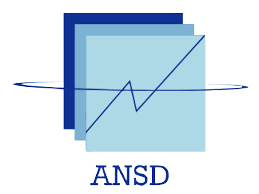
\includegraphics[width=4cm]{Logo3.png} \\[0.1cm]  
        
        \textbf{\large École Nationale de la Statistique et de l'Analyse Économique Pierre Ndiaye (ENSAE)}\\[0.4cm]
        
\includegraphics[width=3cm]{Logo4.png} \\[0.1cm]
        
        \textbf{\LARGE PROJET STATISTIQUES SOUS R }\\[0.3cm]
        \textbf{\Huge \color{black} \textsf{TP1 : Documentation en Rmarkdown}}\\[0.2cm]
        \rule{\linewidth}{0.2mm} \\[0.5cm]
        
        \begin{minipage}{0.5\textwidth}
    \begin{flushleft} \large
        \emph{\textsf{Rédigé par :}}\\
        \textbf{Mame Balla BOUSSO}\\
        \textbf{Ameth FAYE}\\
        \textbf{EDIMA Biyenda Hildégarde}\\
        \textbf{Papa Amadou NIANG}\\
        \textit{Elèves ingénieurs statisticiens économistes}
    \end{flushleft}
\end{minipage}
        \hfill
        \begin{minipage}{0.4\textwidth}
            \begin{flushright} \large
                \emph{\textsf{Sous la supervision de :}} \\
                \textbf{M. Aboubacar HEMA}\\
                \textit{ANALYSTE DE RECHERCHE CHEZ IFPRI }
            \end{flushright}
        \end{minipage}

        \vfill

        {\large \textsf{Année scolaire : 2024/2025}}\\[0.5cm]
        
    \end{center}
\end{titlepage}

\hypertarget{i.-introduction-et-prise-en-main}{%
\section{I. Introduction et prise en
main}\label{i.-introduction-et-prise-en-main}}

\hypertarget{quest-ce-que-r-markdown}{%
\subsection{Qu'est-ce que R Markdown ?}\label{quest-ce-que-r-markdown}}

\hypertarget{duxe9finition}{%
\subsubsection{Définition :}\label{duxe9finition}}

R Markdown est un format de document dynamique qui permet d'intégrer du
code R avec du texte explicatif dans un même fichier. Il est basé sur la
syntaxe Markdown, une syntaxe légère pour le formatage de texte, et il
utilise des outils comme \texttt{knitr} et \texttt{pandoc} pour générer
des rapports, des présentations, et même des sites web.

\hypertarget{avantages-de-r-markdown}{%
\subsubsection{Avantages de R Markdown
:}\label{avantages-de-r-markdown}}

\begin{itemize}
\tightlist
\item
  \textbf{Reproductibilité} : Générer des rapports automatiques et
  reproductibles.
\item
  \textbf{Formats variés} : Peut être converti en HTML, PDF, Word, etc.
\item
  \textbf{Intégration de code} : Permet d'exécuter du code R directement
  dans le document.
\item
  \textbf{Automatisation} : Idéal pour les rapports récurrents.
\item
  \textbf{Clarté} : Séparation du code et du texte explicatif.
\end{itemize}

\hypertarget{pourquoi-utiliser-r-markdown}{%
\subsection{Pourquoi utiliser R Markdown
?}\label{pourquoi-utiliser-r-markdown}}

R Markdown est particulièrement utile dans le domaine des statistiques
et de l'analyse de données, car il permet de combiner la puissance de R
pour le traitement des données avec une présentation claire et
structurée des résultats. Que vous souhaitiez créer des rapports
académiques, des analyses de données interactives ou des présentations
professionnelles, R Markdown offre la flexibilité nécessaire pour
répondre à vos besoins.

\hypertarget{ii.-les-bases-de-r-markdown}{%
\section{II. Les bases de R
Markdown}\label{ii.-les-bases-de-r-markdown}}

\hypertarget{syntaxe-markdown}{%
\subsection{1. Syntaxe Markdown}\label{syntaxe-markdown}}

R Markdown repose sur Markdown, qui permet d'écrire du texte en
utilisant une syntaxe simple pour la mise en forme.

\hypertarget{a-mise-en-forme-inline-italique-gras-liens-etc.}{%
\subsubsection{a) Mise en forme inline (italique, gras, liens,
etc.)}\label{a-mise-en-forme-inline-italique-gras-liens-etc.}}

Voici quelques exemples de mise en forme :

\begin{itemize}
\tightlist
\item
  \textbf{Italique} :
\end{itemize}

\begin{Shaded}
\begin{Highlighting}[]
\FunctionTok{cat}\NormalTok{(}\StringTok{"*Texte en italique* ou \_Texte en italique\_"}\NormalTok{)}
\end{Highlighting}
\end{Shaded}

\begin{verbatim}
## *Texte en italique* ou _Texte en italique_
\end{verbatim}

\emph{Texte en italique} ou \emph{Texte en italique}

\begin{itemize}
\tightlist
\item
  \textbf{Gras} :
\end{itemize}

\begin{Shaded}
\begin{Highlighting}[]
\FunctionTok{cat}\NormalTok{(}\StringTok{"**Texte en gras** ou \_\_Texte en gras\_\_"}\NormalTok{)}
\end{Highlighting}
\end{Shaded}

\begin{verbatim}
## **Texte en gras** ou __Texte en gras__
\end{verbatim}

\textbf{Texte en gras} ou \textbf{Texte en gras}

\begin{itemize}
\tightlist
\item
  \textbf{Lien} :
\end{itemize}

\begin{Shaded}
\begin{Highlighting}[]
\FunctionTok{cat}\NormalTok{(}\StringTok{"[Nom du lien](https://github.com/Abson{-}dev/Projet{-}statistique{-}sous{-}R)"}\NormalTok{)}
\end{Highlighting}
\end{Shaded}

\begin{verbatim}
## [Nom du lien](https://github.com/Abson-dev/Projet-statistique-sous-R)
\end{verbatim}

\href{https://github.com/Abson-dev/Projet-statistique-sous-R}{Nom du
lien}

\hypertarget{b-uxe9luxe9ments-de-niveau-bloc-titres-listes-citations}{%
\subsubsection{b) Éléments de niveau bloc (titres, listes,
citations\ldots)}\label{b-uxe9luxe9ments-de-niveau-bloc-titres-listes-citations}}

\begin{itemize}
\tightlist
\item
  \textbf{Titres} :
\end{itemize}

\begin{Shaded}
\begin{Highlighting}[]
\FunctionTok{cat}\NormalTok{(}\StringTok{"\# Titre de niveau 1}\SpecialCharTok{\textbackslash{}n}\StringTok{\#\# Titre de niveau 2}\SpecialCharTok{\textbackslash{}n}\StringTok{\#\#\# Titre de niveau 3"}\NormalTok{)}
\end{Highlighting}
\end{Shaded}

\hypertarget{titre-de-niveau-1}{%
\section{Titre de niveau 1}\label{titre-de-niveau-1}}

\hypertarget{titre-de-niveau-2}{%
\subsection{Titre de niveau 2}\label{titre-de-niveau-2}}

\hypertarget{titre-de-niveau-3}{%
\subsubsection{Titre de niveau 3}\label{titre-de-niveau-3}}

\begin{itemize}
\tightlist
\item
  \textbf{Listes à puces} :
\end{itemize}

\begin{Shaded}
\begin{Highlighting}[]
\FunctionTok{cat}\NormalTok{(}\StringTok{"{-} Élément 1}\SpecialCharTok{\textbackslash{}n}\StringTok{{-} Élément 2}\SpecialCharTok{\textbackslash{}n}\StringTok{  {-} Sous{-}élément 2.1"}\NormalTok{)}
\end{Highlighting}
\end{Shaded}

\begin{itemize}
\tightlist
\item
  Élément 1
\item
  Élément 2

  \begin{itemize}
  \tightlist
  \item
    Sous-élément 2.1
  \end{itemize}
\item
  Élément 1
\item
  Élément 2

  \begin{itemize}
  \tightlist
  \item
    Sous-élément 2.1
  \end{itemize}
\item
  \textbf{Listes numérotées} :
\end{itemize}

\begin{Shaded}
\begin{Highlighting}[]
\FunctionTok{cat}\NormalTok{(}\StringTok{"1. Premier point}\SpecialCharTok{\textbackslash{}n}\StringTok{2. Deuxième point"}\NormalTok{)}
\end{Highlighting}
\end{Shaded}

\begin{enumerate}
\def\labelenumi{\arabic{enumi}.}
\item
  Premier point
\item
  Deuxième point
\item
  Premier point
\item
  Deuxième point
\end{enumerate}

\begin{itemize}
\tightlist
\item
  \textbf{Citations} :
\end{itemize}

\begin{Shaded}
\begin{Highlighting}[]
\FunctionTok{cat}\NormalTok{(}\StringTok{"\textgreater{} Ceci est une citation"}\NormalTok{)}
\end{Highlighting}
\end{Shaded}

\begin{quote}
Ceci est une citation
\end{quote}

\begin{quote}
Ceci est une citation
\end{quote}

\hypertarget{c-expressions-mathuxe9matiques}{%
\subsubsection{c) Expressions
mathématiques}\label{c-expressions-mathuxe9matiques}}

R Markdown permet d'intégrer des équations LaTeX pour les formules
mathématiques :

-Binôme de Newton

\begin{Shaded}
\begin{Highlighting}[]
\FunctionTok{cat}\NormalTok{(}\StringTok{"Le théorème du binôme de Newton s\textquotesingle{}écrit comme suit :}\SpecialCharTok{\textbackslash{}n\textbackslash{}n}\StringTok{"}\NormalTok{)}
\end{Highlighting}
\end{Shaded}

Le théorème du binôme de Newton s'écrit comme suit :

\begin{Shaded}
\begin{Highlighting}[]
\FunctionTok{cat}\NormalTok{(}\StringTok{"$$ (a + b)\^{}n = }\SpecialCharTok{\textbackslash{}\textbackslash{}}\StringTok{sum\_\{k=0\}\^{}\{n\} }\SpecialCharTok{\textbackslash{}\textbackslash{}}\StringTok{binom\{n\}\{k\} a\^{}\{n{-}k\} b\^{}k $$}\SpecialCharTok{\textbackslash{}n\textbackslash{}n}\StringTok{"}\NormalTok{)}
\end{Highlighting}
\end{Shaded}

\[ (a + b)^n = \sum_{k=0}^{n} \binom{n}{k} a^{n-k} b^k \] -Fonction
continue

\begin{Shaded}
\begin{Highlighting}[]
\FunctionTok{cat}\NormalTok{(}\StringTok{"Une fonction }\SpecialCharTok{\textbackslash{}\textbackslash{}}\StringTok{( f }\SpecialCharTok{\textbackslash{}\textbackslash{}}\StringTok{) est continue en un point }\SpecialCharTok{\textbackslash{}\textbackslash{}}\StringTok{( x\_0 }\SpecialCharTok{\textbackslash{}\textbackslash{}}\StringTok{) si :}\SpecialCharTok{\textbackslash{}n\textbackslash{}n}\StringTok{"}\NormalTok{)}
\end{Highlighting}
\end{Shaded}

Une fonction \(f\) est continue en un point \(x_0\) si :

\begin{Shaded}
\begin{Highlighting}[]
\FunctionTok{cat}\NormalTok{(}\StringTok{"$$ }\SpecialCharTok{\textbackslash{}\textbackslash{}}\StringTok{lim\_\{x }\SpecialCharTok{\textbackslash{}\textbackslash{}}\StringTok{to x\_0\} f(x) = f(x\_0) $$}\SpecialCharTok{\textbackslash{}n\textbackslash{}n}\StringTok{"}\NormalTok{)}
\end{Highlighting}
\end{Shaded}

\[ \lim_{x \to x_0} f(x) = f(x_0) \] -Topologie

\begin{Shaded}
\begin{Highlighting}[]
\FunctionTok{cat}\NormalTok{(}\StringTok{"Dans un espace métrique }\SpecialCharTok{\textbackslash{}\textbackslash{}}\StringTok{( (E, d) }\SpecialCharTok{\textbackslash{}\textbackslash{}}\StringTok{), la boule ouverte de centre }\SpecialCharTok{\textbackslash{}\textbackslash{}}\StringTok{( a }\SpecialCharTok{\textbackslash{}\textbackslash{}}\StringTok{) et de rayon }\SpecialCharTok{\textbackslash{}\textbackslash{}}\StringTok{( r \textgreater{} 0 }\SpecialCharTok{\textbackslash{}\textbackslash{}}\StringTok{) est définie par :}\SpecialCharTok{\textbackslash{}n\textbackslash{}n}\StringTok{"}\NormalTok{)}
\end{Highlighting}
\end{Shaded}

Dans un espace métrique \((E, d)\), la boule ouverte de centre \(a\) et
de rayon \(r > 0\) est définie par :

\begin{Shaded}
\begin{Highlighting}[]
\FunctionTok{cat}\NormalTok{(}\StringTok{"$$ B(a, r) = }\SpecialCharTok{\textbackslash{}\textbackslash{}}\StringTok{\{ x }\SpecialCharTok{\textbackslash{}\textbackslash{}}\StringTok{in E }\SpecialCharTok{\textbackslash{}\textbackslash{}}\StringTok{mid d(x, a) \textless{} r }\SpecialCharTok{\textbackslash{}\textbackslash{}}\StringTok{\} $$}\SpecialCharTok{\textbackslash{}n\textbackslash{}n}\StringTok{"}\NormalTok{)}
\end{Highlighting}
\end{Shaded}

\[ B(a, r) = \{ x \in E \mid d(x, a) < r \} \]

-Equations différentielles

\begin{Shaded}
\begin{Highlighting}[]
\FunctionTok{cat}\NormalTok{(}\StringTok{"Une équation différentielle d\textquotesingle{}ordre }\SpecialCharTok{\textbackslash{}\textbackslash{}}\StringTok{( n }\SpecialCharTok{\textbackslash{}\textbackslash{}}\StringTok{) s\textquotesingle{}exprime sous la forme générale :}\SpecialCharTok{\textbackslash{}n\textbackslash{}n}\StringTok{"}\NormalTok{)}
\end{Highlighting}
\end{Shaded}

Une équation différentielle d'ordre \(n\) s'exprime sous la forme
générale :

\begin{Shaded}
\begin{Highlighting}[]
\FunctionTok{cat}\NormalTok{(}\StringTok{"$$ F }\SpecialCharTok{\textbackslash{}\textbackslash{}}\StringTok{left( x, y, }\SpecialCharTok{\textbackslash{}\textbackslash{}}\StringTok{frac\{dy\}\{dx\}, }\SpecialCharTok{\textbackslash{}\textbackslash{}}\StringTok{frac\{d\^{}2y\}\{dx\^{}2\}, }\SpecialCharTok{\textbackslash{}\textbackslash{}}\StringTok{dots, }\SpecialCharTok{\textbackslash{}\textbackslash{}}\StringTok{frac\{d\^{}ny\}\{dx\^{}n\} }\SpecialCharTok{\textbackslash{}\textbackslash{}}\StringTok{right) = 0 $$}\SpecialCharTok{\textbackslash{}n\textbackslash{}n}\StringTok{"}\NormalTok{)}
\end{Highlighting}
\end{Shaded}

\[ F \left( x, y, \frac{dy}{dx}, \frac{d^2y}{dx^2}, \dots, \frac{d^ny}{dx^n} \right) = 0 \]
-Théorie des sondages

\begin{Shaded}
\begin{Highlighting}[]
\FunctionTok{cat}\NormalTok{(}\StringTok{"Dans la théorie des sondages, l\textquotesingle{}estimateur de la moyenne de la population est donné par :}\SpecialCharTok{\textbackslash{}n\textbackslash{}n}\StringTok{"}\NormalTok{)}
\end{Highlighting}
\end{Shaded}

Dans la théorie des sondages, l'estimateur de la moyenne de la
population est donné par :

\begin{Shaded}
\begin{Highlighting}[]
\FunctionTok{cat}\NormalTok{(}\StringTok{"$$ }\SpecialCharTok{\textbackslash{}\textbackslash{}}\StringTok{bar\{y\} = }\SpecialCharTok{\textbackslash{}\textbackslash{}}\StringTok{frac\{1\}\{n\} }\SpecialCharTok{\textbackslash{}\textbackslash{}}\StringTok{sum\_\{i=1\}\^{}\{n\} y\_i $$}\SpecialCharTok{\textbackslash{}n\textbackslash{}n}\StringTok{"}\NormalTok{)}
\end{Highlighting}
\end{Shaded}

\[ \bar{y} = \frac{1}{n} \sum_{i=1}^{n} y_i \]

-Algèbre linéaire

\begin{Shaded}
\begin{Highlighting}[]
\FunctionTok{cat}\NormalTok{(}\StringTok{"En algèbre linéaire, une matrice }\SpecialCharTok{\textbackslash{}\textbackslash{}}\StringTok{( A }\SpecialCharTok{\textbackslash{}\textbackslash{}}\StringTok{) de dimension }\SpecialCharTok{\textbackslash{}\textbackslash{}}\StringTok{( m }\SpecialCharTok{\textbackslash{}\textbackslash{}}\StringTok{times n }\SpecialCharTok{\textbackslash{}\textbackslash{}}\StringTok{) est représentée sous la forme suivante :}\SpecialCharTok{\textbackslash{}n\textbackslash{}n}\StringTok{"}\NormalTok{)}
\end{Highlighting}
\end{Shaded}

En algèbre linéaire, une matrice \(A\) de dimension \(m \times n\) est
représentée sous la forme suivante :

\begin{Shaded}
\begin{Highlighting}[]
\FunctionTok{cat}\NormalTok{(}\StringTok{"$$ A = }\SpecialCharTok{\textbackslash{}\textbackslash{}}\StringTok{begin\{bmatrix\} }
\StringTok{a\_\{11\} \& a\_\{12\} \& }\SpecialCharTok{\textbackslash{}\textbackslash{}}\StringTok{cdots \& a\_\{1n\} }\SpecialCharTok{\textbackslash{}\textbackslash{}\textbackslash{}\textbackslash{}}\StringTok{ }
\StringTok{a\_\{21\} \& a\_\{22\} \& }\SpecialCharTok{\textbackslash{}\textbackslash{}}\StringTok{cdots \& a\_\{2n\} }\SpecialCharTok{\textbackslash{}\textbackslash{}\textbackslash{}\textbackslash{}}\StringTok{ }
\SpecialCharTok{\textbackslash{}\textbackslash{}}\StringTok{vdots \& }\SpecialCharTok{\textbackslash{}\textbackslash{}}\StringTok{vdots \& }\SpecialCharTok{\textbackslash{}\textbackslash{}}\StringTok{ddots \& }\SpecialCharTok{\textbackslash{}\textbackslash{}}\StringTok{vdots }\SpecialCharTok{\textbackslash{}\textbackslash{}\textbackslash{}\textbackslash{}}\StringTok{ }
\StringTok{a\_\{m1\} \& a\_\{m2\} \& }\SpecialCharTok{\textbackslash{}\textbackslash{}}\StringTok{cdots \& a\_\{mn\} }
\SpecialCharTok{\textbackslash{}\textbackslash{}}\StringTok{end\{bmatrix\} $$}\SpecialCharTok{\textbackslash{}n\textbackslash{}n}\StringTok{"}\NormalTok{)}
\end{Highlighting}
\end{Shaded}

\[ A = \begin{bmatrix} 
a_{11} & a_{12} & \cdots & a_{1n} \\ 
a_{21} & a_{22} & \cdots & a_{2n} \\ 
\vdots & \vdots & \ddots & \vdots \\ 
a_{m1} & a_{m2} & \cdots & a_{mn} 
\end{bmatrix} \] -Probabilités et statistiques

\begin{Shaded}
\begin{Highlighting}[]
\FunctionTok{cat}\NormalTok{(}\StringTok{"L\textquotesingle{}espérance mathématique d\textquotesingle{}une variable aléatoire }\SpecialCharTok{\textbackslash{}\textbackslash{}}\StringTok{( X }\SpecialCharTok{\textbackslash{}\textbackslash{}}\StringTok{) discrète est donnée par :}\SpecialCharTok{\textbackslash{}n\textbackslash{}n}\StringTok{"}\NormalTok{)}
\end{Highlighting}
\end{Shaded}

L'espérance mathématique d'une variable aléatoire \(X\) discrète est
donnée par :

\begin{Shaded}
\begin{Highlighting}[]
\FunctionTok{cat}\NormalTok{(}\StringTok{"$$ }\SpecialCharTok{\textbackslash{}\textbackslash{}}\StringTok{mathbb\{E\}[X] = }\SpecialCharTok{\textbackslash{}\textbackslash{}}\StringTok{sum\_\{i=1\}\^{}\{n\} x\_i P(x\_i) $$}\SpecialCharTok{\textbackslash{}n\textbackslash{}n}\StringTok{"}\NormalTok{)}
\end{Highlighting}
\end{Shaded}

\[ \mathbb{E}[X] = \sum_{i=1}^{n} x_i P(x_i) \]

\begin{Shaded}
\begin{Highlighting}[]
\FunctionTok{cat}\NormalTok{(}\StringTok{"La variance est définie comme suit :}\SpecialCharTok{\textbackslash{}n\textbackslash{}n}\StringTok{"}\NormalTok{)}
\end{Highlighting}
\end{Shaded}

La variance est définie comme suit :

\begin{Shaded}
\begin{Highlighting}[]
\FunctionTok{cat}\NormalTok{(}\StringTok{"$$ }\SpecialCharTok{\textbackslash{}\textbackslash{}}\StringTok{text\{Var\}(X) = }\SpecialCharTok{\textbackslash{}\textbackslash{}}\StringTok{mathbb\{E\}[X\^{}2] {-} (}\SpecialCharTok{\textbackslash{}\textbackslash{}}\StringTok{mathbb\{E\}[X])\^{}2 $$}\SpecialCharTok{\textbackslash{}n\textbackslash{}n}\StringTok{"}\NormalTok{)}
\end{Highlighting}
\end{Shaded}

\[ \text{Var}(X) = \mathbb{E}[X^2] - (\mathbb{E}[X])^2 \]

-Séries de Fourrier

\begin{Shaded}
\begin{Highlighting}[]
\FunctionTok{cat}\NormalTok{(}\StringTok{"La décomposition en série de Fourier d\textquotesingle{}une fonction périodique }\SpecialCharTok{\textbackslash{}\textbackslash{}}\StringTok{( f(x) }\SpecialCharTok{\textbackslash{}\textbackslash{}}\StringTok{) est donnée par :}\SpecialCharTok{\textbackslash{}n\textbackslash{}n}\StringTok{"}\NormalTok{)}
\end{Highlighting}
\end{Shaded}

La décomposition en série de Fourier d'une fonction périodique \(f(x)\)
est donnée par :

\begin{Shaded}
\begin{Highlighting}[]
\FunctionTok{cat}\NormalTok{(}\StringTok{"$$ f(x) = a\_0 + }\SpecialCharTok{\textbackslash{}\textbackslash{}}\StringTok{sum\_\{n=1\}\^{}\{}\SpecialCharTok{\textbackslash{}\textbackslash{}}\StringTok{infty\} }\SpecialCharTok{\textbackslash{}\textbackslash{}}\StringTok{left( a\_n }\SpecialCharTok{\textbackslash{}\textbackslash{}}\StringTok{cos(nx) + b\_n }\SpecialCharTok{\textbackslash{}\textbackslash{}}\StringTok{sin(nx) }\SpecialCharTok{\textbackslash{}\textbackslash{}}\StringTok{right) $$}\SpecialCharTok{\textbackslash{}n\textbackslash{}n}\StringTok{"}\NormalTok{)}
\end{Highlighting}
\end{Shaded}

\[ f(x) = a_0 + \sum_{n=1}^{\infty} \left( a_n \cos(nx) + b_n \sin(nx) \right) \]

\begin{Shaded}
\begin{Highlighting}[]
\FunctionTok{cat}\NormalTok{(}\StringTok{"Où les coefficients sont définis par :}\SpecialCharTok{\textbackslash{}n\textbackslash{}n}\StringTok{"}\NormalTok{)}
\end{Highlighting}
\end{Shaded}

Où les coefficients sont définis par :

\begin{Shaded}
\begin{Highlighting}[]
\FunctionTok{cat}\NormalTok{(}\StringTok{"$$ a\_n = }\SpecialCharTok{\textbackslash{}\textbackslash{}}\StringTok{frac\{1\}\{}\SpecialCharTok{\textbackslash{}\textbackslash{}}\StringTok{pi\} }\SpecialCharTok{\textbackslash{}\textbackslash{}}\StringTok{int\_\{{-}}\SpecialCharTok{\textbackslash{}\textbackslash{}}\StringTok{pi\}\^{}\{}\SpecialCharTok{\textbackslash{}\textbackslash{}}\StringTok{pi\} f(x) }\SpecialCharTok{\textbackslash{}\textbackslash{}}\StringTok{cos(nx) }\SpecialCharTok{\textbackslash{}\textbackslash{}}\StringTok{, dx $$}\SpecialCharTok{\textbackslash{}n\textbackslash{}n}\StringTok{"}\NormalTok{)}
\end{Highlighting}
\end{Shaded}

\[ a_n = \frac{1}{\pi} \int_{-\pi}^{\pi} f(x) \cos(nx) \, dx \]

\begin{Shaded}
\begin{Highlighting}[]
\FunctionTok{cat}\NormalTok{(}\StringTok{"$$ b\_n = }\SpecialCharTok{\textbackslash{}\textbackslash{}}\StringTok{frac\{1\}\{}\SpecialCharTok{\textbackslash{}\textbackslash{}}\StringTok{pi\} }\SpecialCharTok{\textbackslash{}\textbackslash{}}\StringTok{int\_\{{-}}\SpecialCharTok{\textbackslash{}\textbackslash{}}\StringTok{pi\}\^{}\{}\SpecialCharTok{\textbackslash{}\textbackslash{}}\StringTok{pi\} f(x) }\SpecialCharTok{\textbackslash{}\textbackslash{}}\StringTok{sin(nx) }\SpecialCharTok{\textbackslash{}\textbackslash{}}\StringTok{, dx $$}\SpecialCharTok{\textbackslash{}n\textbackslash{}n}\StringTok{"}\NormalTok{)}
\end{Highlighting}
\end{Shaded}

\[ b_n = \frac{1}{\pi} \int_{-\pi}^{\pi} f(x) \sin(nx) \, dx \]

-Séries de Taylor

\begin{Shaded}
\begin{Highlighting}[]
\FunctionTok{cat}\NormalTok{(}\StringTok{"Le développement en série de Taylor d\textquotesingle{}une fonction }\SpecialCharTok{\textbackslash{}\textbackslash{}}\StringTok{( f(x) }\SpecialCharTok{\textbackslash{}\textbackslash{}}\StringTok{) autour d\textquotesingle{}un point }\SpecialCharTok{\textbackslash{}\textbackslash{}}\StringTok{( a }\SpecialCharTok{\textbackslash{}\textbackslash{}}\StringTok{) est donné par :}\SpecialCharTok{\textbackslash{}n\textbackslash{}n}\StringTok{"}\NormalTok{)}
\end{Highlighting}
\end{Shaded}

Le développement en série de Taylor d'une fonction \(f(x)\) autour d'un
point \(a\) est donné par :

\begin{Shaded}
\begin{Highlighting}[]
\FunctionTok{cat}\NormalTok{(}\StringTok{"$$ f(x) = f(a) + f\textquotesingle{}(a)(x{-}a) + }\SpecialCharTok{\textbackslash{}\textbackslash{}}\StringTok{frac\{f\textquotesingle{}\textquotesingle{}(a)\}\{2!\}(x{-}a)\^{}2 + }\SpecialCharTok{\textbackslash{}\textbackslash{}}\StringTok{dots $$}\SpecialCharTok{\textbackslash{}n\textbackslash{}n}\StringTok{"}\NormalTok{)}
\end{Highlighting}
\end{Shaded}

\[ f(x) = f(a) + f'(a)(x-a) + \frac{f''(a)}{2!}(x-a)^2 + \dots \]

\hypertarget{table-des-matiuxe8res-et-options-globales}{%
\subsection{2. Table des matières et options
globales}\label{table-des-matiuxe8res-et-options-globales}}

Vous pouvez configurer une table des matières et d'autres options
globales en modifiant les métadonnées YAML et le chunk \texttt{setup} au
début du document.

\hypertarget{ajouter-une-table-des-matiuxe8res-et-numuxe9roter-les-sections}{%
\subsubsection{Ajouter une table des matières et numéroter les
sections}\label{ajouter-une-table-des-matiuxe8res-et-numuxe9roter-les-sections}}

Les options pour la table des matières et la numérotation des sections
sont déjà incluses dans les métadonnées YAML :

\begin{Shaded}
\begin{Highlighting}[]
\FunctionTok{output}\KeywordTok{:}
\AttributeTok{  }\FunctionTok{pdf\_document}\KeywordTok{:}
\AttributeTok{    }\FunctionTok{latex\_engine}\KeywordTok{:}\AttributeTok{ xelatex}
\AttributeTok{    }\FunctionTok{keep\_tex}\KeywordTok{:}\AttributeTok{ }\CharTok{true}
\AttributeTok{    }\FunctionTok{toc}\KeywordTok{:}\AttributeTok{ }\CharTok{true}
\AttributeTok{    }\FunctionTok{number\_sections}\KeywordTok{:}\AttributeTok{ }\CharTok{true}
\end{Highlighting}
\end{Shaded}

\hypertarget{iii.-formats-de-sortie-courants}{%
\section{III. Formats de sortie
courants}\label{iii.-formats-de-sortie-courants}}

La version originale de Markdown a été inventée principalement pour
écrire plus facilement du contenu HTML. Par exemple, vous pouvez écrire
une puce avec \texttt{-\ text} au lieu du code HTML détaillé
\texttt{\textless{}ul\textgreater{}\textless{}li\textgreater{}text\textless{}/li\textgreater{}\textless{}/ul\textgreater{}},
ou une citation avec \texttt{\textgreater{}\ text} au lieu de
\texttt{\textless{}blockquote\textgreater{}text\textless{}/blockquote\textgreater{}}.

La syntaxe de Markdown a été considérablement étendue par Pandoc. De
plus, Pandoc permet de convertir un document Markdown en une grande
variété de formats de sortie. Dans cette partie, nous présenterons les
fonctionnalités de divers formats de sortie de document.

\hypertarget{document-html}{%
\subsection{1. Document HTML}\label{document-html}}

Comme nous venons de le mentionner, Markdown a été conçu à l'origine
pour la sortie HTML, il n'est donc pas surprenant que le format HTML
possède les fonctionnalités les plus riches parmi tous les formats de
sortie.

Pour créer un document HTML à partir de R Markdown, vous spécifiez le
\texttt{html\_document} format de sortie dans les métadonnées YAML de
votre document :

\begin{Shaded}
\begin{Highlighting}[]
\PreprocessorTok{{-}{-}{-}}
\FunctionTok{title}\KeywordTok{:}\AttributeTok{ }\StringTok{"Titre du document"}
\FunctionTok{author}\KeywordTok{:}\AttributeTok{ Auteur}
\FunctionTok{date}\KeywordTok{:}\AttributeTok{ La date}
\FunctionTok{output}\KeywordTok{:}\AttributeTok{ html\_document}
\PreprocessorTok{{-}{-}{-}}
\end{Highlighting}
\end{Shaded}

\hypertarget{table-des-matiuxe8res}{%
\subsubsection{1.1 Table des matières}\label{table-des-matiuxe8res}}

Vous pouvez ajouter une table des matières (TOC) à l'aide de l'
\texttt{toc} option et spécifier la profondeur des en-têtes à appliquer
à l'aide de l' \texttt{toc\_depth} option. Par exemple :

\begin{Shaded}
\begin{Highlighting}[]
\PreprocessorTok{{-}{-}{-}}
\FunctionTok{title}\KeywordTok{:}\AttributeTok{ }\StringTok{"Titre du document"}
\FunctionTok{output}\KeywordTok{:}
\AttributeTok{  }\FunctionTok{html\_document}\KeywordTok{:}
\AttributeTok{    }\FunctionTok{toc}\KeywordTok{:}\AttributeTok{ }\CharTok{true}
\AttributeTok{    }\FunctionTok{toc\_depth}\KeywordTok{:}\AttributeTok{ }\DecValTok{2}
\PreprocessorTok{{-}{-}{-}}
\end{Highlighting}
\end{Shaded}

Si la profondeur de la table des matières n'est pas explicitement
spécifiée, la valeur par défaut est 3 (ce qui signifie que tous les
en-têtes de niveau 1, 2 et 3 seront inclus dans la table des matières).

\hypertarget{numuxe9rotation-des-sections}{%
\subsubsection{1.2 Numérotation des
sections}\label{numuxe9rotation-des-sections}}

Vous pouvez ajouter une numérotation de section aux en-têtes à l'aide de
l' \texttt{number\_sections} option :

\begin{Shaded}
\begin{Highlighting}[]
\PreprocessorTok{{-}{-}{-}}
\FunctionTok{title}\KeywordTok{:}\AttributeTok{ }\StringTok{"Titre du document"}
\FunctionTok{output}\KeywordTok{:}
\AttributeTok{  }\FunctionTok{html\_document}\KeywordTok{:}
\AttributeTok{    }\FunctionTok{toc}\KeywordTok{:}\AttributeTok{ }\CharTok{true}
\AttributeTok{    }\FunctionTok{number\_sections}\KeywordTok{:}\AttributeTok{ }\CharTok{true}
\PreprocessorTok{{-}{-}{-}}
\end{Highlighting}
\end{Shaded}

Notez que si vous choisissez d'utiliser cette \texttt{number\_sections}
option, vous souhaiterez probablement également utiliser \texttt{\#} des
en-têtes (H1) dans votre document, car \texttt{\#\#} les en-têtes (H2)
incluront un point décimal, car sans en-têtes H1, vos en-têtes H2 seront
numérotés avec 0.1, 0.2, etc.

\hypertarget{apparence-et-style}{%
\subsubsection{1.3 Apparence et style}\label{apparence-et-style}}

Il existe plusieurs options qui contrôlent l'apparence des documents
HTML :

\begin{itemize}
\item
  \textbf{theme} spécifie le thème Bootstrap à utiliser pour la page
  (les thèmes sont tirés de la bibliothèque de thèmes Bootswatch ). Les
  thèmes valides incluent default, bootstrap, cerulean, cosmo, darkly,
  flatly, journal, lumen, paper, readable, sandstone, simplex, spacelab,
  united et yeti. Ne passez \texttt{null} aucun thème (dans ce cas, vous
  pouvez utiliser le \texttt{css} paramètre pour ajouter vos propres
  styles).
\item
  \textbf{highlight} spécifie le style de mise en surbrillance de la
  syntaxe. Les styles pris en charge incluent default, tango, pygments,
  kate, monochrome, espresso, zenburn, haddock, breezedark, et textmate.
  Passez \texttt{null} pour empêcher la mise en surbrillance de la
  syntaxe.
\item
  \textbf{smart} indique si une sortie typographiquement correcte doit
  être produite, en convertissant les guillemets droits en guillemets
  bouclés, --- en tirets cadratins, -- en tirets demi-cadratins et
  \ldots{} en points de suspension. Notez que cette \texttt{smart}
  option est activée par défaut.
\end{itemize}

Par exemple :

\begin{Shaded}
\begin{Highlighting}[]
\PreprocessorTok{{-}{-}{-}}
\FunctionTok{title}\KeywordTok{:}\AttributeTok{ }\StringTok{"Titre du document"}
\FunctionTok{output}\KeywordTok{:}
\AttributeTok{  }\FunctionTok{html\_document}\KeywordTok{:}
\AttributeTok{    }\FunctionTok{theme}\KeywordTok{:}\AttributeTok{ united}
\AttributeTok{    }\FunctionTok{highlight}\KeywordTok{:}\AttributeTok{ tango}
\PreprocessorTok{{-}{-}{-}}
\end{Highlighting}
\end{Shaded}

\hypertarget{css-personnalisuxe9}{%
\subsubsection{1.4 CSS personnalisé}\label{css-personnalisuxe9}}

Vous pouvez ajouter votre propre CSS à un document HTML en utilisant l'
\texttt{css} option :

\begin{Shaded}
\begin{Highlighting}[]
\PreprocessorTok{{-}{-}{-}}
\FunctionTok{title}\KeywordTok{:}\AttributeTok{ }\StringTok{"Titre du document"}
\FunctionTok{output}\KeywordTok{:}
\AttributeTok{  }\FunctionTok{html\_document}\KeywordTok{:}
\AttributeTok{    }\FunctionTok{css}\KeywordTok{:}\AttributeTok{ styles.css}
\PreprocessorTok{{-}{-}{-}}
\end{Highlighting}
\end{Shaded}

\hypertarget{document-pdf}{%
\subsection{2. Document PDF}\label{document-pdf}}

Pour créer un document PDF à partir de R Markdown, vous spécifiez le
\texttt{pdf\_document} format de sortie dans les métadonnées YAML :

\begin{Shaded}
\begin{Highlighting}[]
\PreprocessorTok{{-}{-}{-}}
\FunctionTok{title}\KeywordTok{:}\AttributeTok{ }\StringTok{"Titre du document"}
\FunctionTok{author}\KeywordTok{:}\AttributeTok{ Auteur}
\FunctionTok{date}\KeywordTok{:}\AttributeTok{ La date}
\FunctionTok{output}\KeywordTok{:}\AttributeTok{ pdf\_document}
\PreprocessorTok{{-}{-}{-}}
\end{Highlighting}
\end{Shaded}

Dans les documents R Markdown qui génèrent une sortie PDF, vous pouvez
utiliser du LaTeX brut et même définir des macros LaTeX. Consultez la
documentation de Pandoc sur l'extension \texttt{raw\_tex} pour plus de
détails.

Notez que la sortie PDF (y compris les diapositives Beamer) nécessite
une installation de LaTeX.

\hypertarget{table-des-matiuxe8res-1}{%
\subsubsection{2.1 Table des matières}\label{table-des-matiuxe8res-1}}

Vous pouvez ajouter une table des matières à l'aide de l' \texttt{toc}
option et spécifier la profondeur des en-têtes à appliquer à l'aide de
l' \texttt{toc\_depth} option. Par exemple :

\begin{Shaded}
\begin{Highlighting}[]
\PreprocessorTok{{-}{-}{-}}
\FunctionTok{title}\KeywordTok{:}\AttributeTok{ }\StringTok{"Titre du document"}
\FunctionTok{output}\KeywordTok{:}
\AttributeTok{  }\FunctionTok{pdf\_document}\KeywordTok{:}
\AttributeTok{    }\FunctionTok{toc}\KeywordTok{:}\AttributeTok{ }\CharTok{true}
\AttributeTok{    }\FunctionTok{toc\_depth}\KeywordTok{:}\AttributeTok{ }\DecValTok{2}
\PreprocessorTok{{-}{-}{-}}
\end{Highlighting}
\end{Shaded}

Si la profondeur de la table des matières n'est pas explicitement
spécifiée, elle est par défaut de 2 (ce qui signifie que tous les
en-têtes de niveau 1 et 2 seront inclus dans la table des matières),
tandis qu'elle est par défaut de 3 dans \texttt{html\_document}.

Vous pouvez ajouter une numérotation de section aux en-têtes à l'aide de
l' \texttt{number\_sections} option :

\begin{Shaded}
\begin{Highlighting}[]
\PreprocessorTok{{-}{-}{-}}
\FunctionTok{title}\KeywordTok{:}\AttributeTok{ }\StringTok{"Titre du document"}
\FunctionTok{output}\KeywordTok{:}
\AttributeTok{  }\FunctionTok{pdf\_document}\KeywordTok{:}
\AttributeTok{    }\FunctionTok{toc}\KeywordTok{:}\AttributeTok{ }\CharTok{true}
\AttributeTok{    }\FunctionTok{number\_sections}\KeywordTok{:}\AttributeTok{ }\CharTok{true}
\PreprocessorTok{{-}{-}{-}}
\end{Highlighting}
\end{Shaded}

Si vous êtes familier avec LaTeX, \texttt{number\_sections:\ true}
signifie \texttt{\textbackslash{}section\{\}}, et
\texttt{number\_sections:\ false} signifie
\texttt{\textbackslash{}section*\{\}} pour les sections dans LaTeX (cela
s'applique également à d'autres niveaux de « sections » tels que
\texttt{\textbackslash{}chapter\{\}}, et
\texttt{\textbackslash{}subsection\{\}}).

\hypertarget{option-latex}{%
\subsubsection{2.2 Option LaTeX}\label{option-latex}}

De nombreux aspects du modèle LaTeX utilisé pour créer des documents PDF
peuvent être personnalisés à l'aide de métadonnées YAML de niveau
supérieur (notez que ces options n'apparaissent pas sous la section
\texttt{output}, mais apparaissent plutôt au niveau supérieur avec
\texttt{title}, \texttt{author}, etc.). Par exemple :

\begin{Shaded}
\begin{Highlighting}[]
\PreprocessorTok{{-}{-}{-}}
\FunctionTok{title}\KeywordTok{:}\AttributeTok{ }\StringTok{"Titre du document"}
\FunctionTok{output}\KeywordTok{:}\AttributeTok{ pdf\_document}
\FunctionTok{fontsize}\KeywordTok{:}\AttributeTok{ 11pt}
\FunctionTok{geometry}\KeywordTok{:}\AttributeTok{ margin=1in}
\PreprocessorTok{{-}{-}{-}}
\end{Highlighting}
\end{Shaded}

\hypertarget{document-word}{%
\subsection{3. Document Word}\label{document-word}}

Pour créer un document Word à partir de R Markdown, vous spécifiez le
\texttt{word\_document} format de sortie dans les métadonnées YAML de
votre document :

\begin{Shaded}
\begin{Highlighting}[]
\PreprocessorTok{{-}{-}{-}}
\FunctionTok{title}\KeywordTok{:}\AttributeTok{ }\StringTok{"Titre du document"}
\FunctionTok{author}\KeywordTok{:}\AttributeTok{ Auteur}
\FunctionTok{date}\KeywordTok{:}\AttributeTok{ La date}
\FunctionTok{output}\KeywordTok{:}\AttributeTok{ word\_document}
\PreprocessorTok{{-}{-}{-}}
\end{Highlighting}
\end{Shaded}

La fonctionnalité la plus remarquable des documents Word est le modèle
Word, également connu sous le nom de « document de référence de style ».
Vous pouvez spécifier un document à utiliser comme référence de style
lors de la production d'un \texttt{*.docx} fichier (un document Word).
Cela vous permettra de personnaliser des éléments tels que les marges et
d'autres caractéristiques de mise en forme. Pour de meilleurs résultats,
le document de référence doit être une version modifiée d'un
\texttt{.docx} fichier produit à l'aide de \texttt{rmarkdown} ou de
Pandoc. Le chemin d'accès d'un tel document peut être passé à l'
\texttt{reference\_docx} argument du \texttt{word\_document} format.
Passez \texttt{"default"} pour utiliser les styles par défaut. Par
exemple :

\begin{Shaded}
\begin{Highlighting}[]
\PreprocessorTok{{-}{-}{-}}
\FunctionTok{title}\KeywordTok{:}\AttributeTok{ }\StringTok{"Titre du document"}
\FunctionTok{author}\KeywordTok{:}\AttributeTok{ Auteur}
\FunctionTok{date}\KeywordTok{:}\AttributeTok{ La date}
\FunctionTok{output}\KeywordTok{:}\AttributeTok{ }
\AttributeTok{  }\FunctionTok{word\_document}\KeywordTok{:}
\AttributeTok{    }\FunctionTok{reference\_docx}\KeywordTok{:}\AttributeTok{ }\StringTok{"mon\_modele.docx"}
\PreprocessorTok{{-}{-}{-}}
\end{Highlighting}
\end{Shaded}

\hypertarget{iv.-cruxe9ation-et-manipulation-de-bases-de-donnuxe9es-fictives}{%
\section{IV. Création et manipulation de bases de données
fictives}\label{iv.-cruxe9ation-et-manipulation-de-bases-de-donnuxe9es-fictives}}

Pour illustrer les concepts de R Markdown, nous allons créer une base de
données fictive qui servira de base pour nos tableaux, graphiques et
équations statistiques. Cette base de données représentera un
échantillon de données démographiques et économiques.

\hypertarget{cruxe9ation-de-la-base-de-donnuxe9es}{%
\subsection{1. Création de la base de
données}\label{cruxe9ation-de-la-base-de-donnuxe9es}}

Nous allons créer un dataframe nommé \texttt{df\_fictif} contenant les
variables suivantes :

\begin{itemize}
\tightlist
\item
  \textbf{ID} : Identifiant unique de l'individu.
\item
  \textbf{Age} : Âge de l'individu.
\item
  \textbf{Sexe} : Sexe de l'individu (Homme/Femme).
\item
  \textbf{Revenu} : Revenu mensuel.
\item
  \textbf{Education} : Niveau d'éducation (Primaire, Secondaire,
  Universitaire).
\item
  \textbf{Ville} : Ville de résidence (Ville A, Ville B, Ville C).
\item
  \textbf{Nombre\_Enfants} : Nombre d'enfants.
\end{itemize}

\begin{Shaded}
\begin{Highlighting}[]
\CommentTok{\# Chargement des packages nécessaires}
\FunctionTok{library}\NormalTok{(dplyr)}
\FunctionTok{library}\NormalTok{(ggplot2)}
\FunctionTok{library}\NormalTok{(knitr)}
\FunctionTok{library}\NormalTok{(kableExtra)}
\FunctionTok{library}\NormalTok{(tidyr)}
\FunctionTok{library}\NormalTok{(xtable)}

\FunctionTok{set.seed}\NormalTok{(}\DecValTok{42}\NormalTok{)  }\CommentTok{\# Pour la reproductibilité}

\CommentTok{\# Création du dataframe}
\NormalTok{df\_fictif }\OtherTok{\textless{}{-}} \FunctionTok{data.frame}\NormalTok{(}
  \AttributeTok{ID =} \DecValTok{1}\SpecialCharTok{:}\DecValTok{500}\NormalTok{,}
  \AttributeTok{Age =} \FunctionTok{sample}\NormalTok{(}\DecValTok{18}\SpecialCharTok{:}\DecValTok{65}\NormalTok{, }\DecValTok{500}\NormalTok{, }\AttributeTok{replace =} \ConstantTok{TRUE}\NormalTok{),}
  \AttributeTok{Sexe =} \FunctionTok{sample}\NormalTok{(}\FunctionTok{c}\NormalTok{(}\StringTok{"Homme"}\NormalTok{, }\StringTok{"Femme"}\NormalTok{), }\DecValTok{500}\NormalTok{, }\AttributeTok{replace =} \ConstantTok{TRUE}\NormalTok{, }\AttributeTok{prob =} \FunctionTok{c}\NormalTok{(}\FloatTok{0.49}\NormalTok{, }\FloatTok{0.51}\NormalTok{)),}
  \AttributeTok{Revenu =} \FunctionTok{round}\NormalTok{(}\FunctionTok{rnorm}\NormalTok{(}\DecValTok{500}\NormalTok{, }\AttributeTok{mean =} \DecValTok{3000}\NormalTok{, }\AttributeTok{sd =} \DecValTok{800}\NormalTok{), }\DecValTok{2}\NormalTok{),}
  \AttributeTok{Education =} \FunctionTok{sample}\NormalTok{(}\FunctionTok{c}\NormalTok{(}\StringTok{"Primaire"}\NormalTok{, }\StringTok{"Secondaire"}\NormalTok{, }\StringTok{"Universitaire"}\NormalTok{), }\DecValTok{500}\NormalTok{, }\AttributeTok{replace =} \ConstantTok{TRUE}\NormalTok{, }\AttributeTok{prob =} \FunctionTok{c}\NormalTok{(}\FloatTok{0.3}\NormalTok{, }\FloatTok{0.5}\NormalTok{, }\FloatTok{0.2}\NormalTok{)),}
  \AttributeTok{Ville =} \FunctionTok{sample}\NormalTok{(}\FunctionTok{c}\NormalTok{(}\StringTok{"Ville A"}\NormalTok{, }\StringTok{"Ville B"}\NormalTok{, }\StringTok{"Ville C"}\NormalTok{), }\DecValTok{500}\NormalTok{, }\AttributeTok{replace =} \ConstantTok{TRUE}\NormalTok{, }\AttributeTok{prob =} \FunctionTok{c}\NormalTok{(}\FloatTok{0.4}\NormalTok{, }\FloatTok{0.35}\NormalTok{, }\FloatTok{0.25}\NormalTok{)),}
  \AttributeTok{Nombre\_Enfants =} \FunctionTok{sample}\NormalTok{(}\DecValTok{0}\SpecialCharTok{:}\DecValTok{5}\NormalTok{, }\DecValTok{500}\NormalTok{, }\AttributeTok{replace =} \ConstantTok{TRUE}\NormalTok{, }\AttributeTok{prob =} \FunctionTok{c}\NormalTok{(}\FloatTok{0.3}\NormalTok{, }\FloatTok{0.25}\NormalTok{, }\FloatTok{0.2}\NormalTok{, }\FloatTok{0.15}\NormalTok{, }\FloatTok{0.07}\NormalTok{, }\FloatTok{0.03}\NormalTok{))}
\NormalTok{)}

\CommentTok{\# Visualisation des premières lignes}
\FunctionTok{head}\NormalTok{(df\_fictif)}
\end{Highlighting}
\end{Shaded}

\begin{verbatim}
##   ID Age  Sexe  Revenu  Education   Ville Nombre_Enfants
## 1  1  54 Homme 2443.58 Secondaire Ville A              3
## 2  2  18 Homme 2719.92 Secondaire Ville B              4
## 3  3  42 Femme 2848.79   Primaire Ville A              0
## 4  4  27 Homme 3390.21   Primaire Ville A              0
## 5  5  53 Femme 3890.67 Secondaire Ville A              0
## 6  6  35 Femme 1219.94 Secondaire Ville A              0
\end{verbatim}

\hypertarget{aperuxe7u-de-la-base-de-donnuxe9es}{%
\subsection{2. Aperçu de la base de
données}\label{aperuxe7u-de-la-base-de-donnuxe9es}}

\begin{longtable}[t]{rrlrllr}
\caption{\label{tab:aperçu-base}Aperçu de la base de données fictive}\\
\toprule
ID & Age & Sexe & Revenu & Education & Ville & Nombre\_Enfants\\
\midrule
1 & 54 & Homme & 2443.58 & Secondaire & Ville A & 3\\
2 & 18 & Homme & 2719.92 & Secondaire & Ville B & 4\\
3 & 42 & Femme & 2848.79 & Primaire & Ville A & 0\\
4 & 27 & Homme & 3390.21 & Primaire & Ville A & 0\\
5 & 53 & Femme & 3890.67 & Secondaire & Ville A & 0\\
\addlinespace
6 & 35 & Femme & 1219.94 & Secondaire & Ville A & 0\\
\bottomrule
\end{longtable}

\hypertarget{ruxe9sumuxe9-statistique}{%
\subsection{3. Résumé statistique}\label{ruxe9sumuxe9-statistique}}

Obtenons un résumé statistique des variables numériques de notre base de
données.

\begin{Shaded}
\begin{Highlighting}[]
\FunctionTok{summary}\NormalTok{(df\_fictif)}
\end{Highlighting}
\end{Shaded}

\begin{verbatim}
##        ID             Age            Sexe               Revenu      
##  Min.   :  1.0   Min.   :18.00   Length:500         Min.   : 631.3  
##  1st Qu.:125.8   1st Qu.:31.00   Class :character   1st Qu.:2447.5  
##  Median :250.5   Median :43.00   Mode  :character   Median :3050.3  
##  Mean   :250.5   Mean   :42.39                      Mean   :3043.5  
##  3rd Qu.:375.2   3rd Qu.:54.00                      3rd Qu.:3576.4  
##  Max.   :500.0   Max.   :65.00                      Max.   :5557.7  
##   Education            Ville           Nombre_Enfants 
##  Length:500         Length:500         Min.   :0.000  
##  Class :character   Class :character   1st Qu.:0.000  
##  Mode  :character   Mode  :character   Median :1.000  
##                                        Mean   :1.634  
##                                        3rd Qu.:3.000  
##                                        Max.   :5.000
\end{verbatim}

\hypertarget{v.-travailler-avec-des-tableaux-en-r-markdown}{%
\section{V. Travailler avec des tableaux en R
Markdown}\label{v.-travailler-avec-des-tableaux-en-r-markdown}}

Les tableaux sont essentiels pour présenter des données de manière
claire et structurée. R Markdown offre plusieurs moyens de créer et de
styliser des tableaux.

\hypertarget{tableaux-simples-avec-knitrkable}{%
\subsection{\texorpdfstring{1. Tableaux simples avec
\texttt{knitr::kable}}{1. Tableaux simples avec knitr::kable}}\label{tableaux-simples-avec-knitrkable}}

La fonction \texttt{kable} du package \texttt{knitr} permet de créer des
tableaux simples et esthétiques.

\begin{Shaded}
\begin{Highlighting}[]
\FunctionTok{kable}\NormalTok{(}\FunctionTok{head}\NormalTok{(df\_fictif, }\DecValTok{10}\NormalTok{), }\AttributeTok{caption =} \StringTok{"Tableau simple des 10 premières entrées"}\NormalTok{) }\SpecialCharTok{\%\textgreater{}\%}
  \FunctionTok{kable\_styling}\NormalTok{(}\AttributeTok{full\_width =} \ConstantTok{FALSE}\NormalTok{, }\AttributeTok{position =} \StringTok{"center"}\NormalTok{)}
\end{Highlighting}
\end{Shaded}

\begin{longtable}[t]{rrlrllr}
\caption{\label{tab:tableau-simple}Tableau simple des 10 premières entrées}\\
\toprule
ID & Age & Sexe & Revenu & Education & Ville & Nombre\_Enfants\\
\midrule
1 & 54 & Homme & 2443.58 & Secondaire & Ville A & 3\\
2 & 18 & Homme & 2719.92 & Secondaire & Ville B & 4\\
3 & 42 & Femme & 2848.79 & Primaire & Ville A & 0\\
4 & 27 & Homme & 3390.21 & Primaire & Ville A & 0\\
5 & 53 & Femme & 3890.67 & Secondaire & Ville A & 0\\
\addlinespace
6 & 35 & Femme & 1219.94 & Secondaire & Ville A & 0\\
7 & 64 & Homme & 4544.80 & Secondaire & Ville B & 0\\
8 & 41 & Femme & 5042.01 & Secondaire & Ville A & 0\\
9 & 24 & Femme & 2072.04 & Primaire & Ville A & 2\\
10 & 53 & Femme & 2433.14 & Secondaire & Ville A & 1\\
\bottomrule
\end{longtable}

\hypertarget{tableaux-avancuxe9s-avec-kableextra}{%
\subsection{\texorpdfstring{2. Tableaux avancés avec
\texttt{kableExtra}}{2. Tableaux avancés avec kableExtra}}\label{tableaux-avancuxe9s-avec-kableextra}}

Le package \texttt{kableExtra} permet d'ajouter des fonctionnalités
avancées aux tableaux créés avec \texttt{kable}.

\hypertarget{a-ajouter-des-lignes-de-suxe9paration-et-des-couleurs}{%
\subsubsection{a) Ajouter des lignes de séparation et des
couleurs}\label{a-ajouter-des-lignes-de-suxe9paration-et-des-couleurs}}

\begin{Shaded}
\begin{Highlighting}[]
\FunctionTok{kable}\NormalTok{(}\FunctionTok{head}\NormalTok{(df\_fictif, }\DecValTok{10}\NormalTok{), }\StringTok{"latex"}\NormalTok{, }\AttributeTok{booktabs =} \ConstantTok{TRUE}\NormalTok{, }\AttributeTok{caption =} \StringTok{"Tableau avancé avec kableExtra"}\NormalTok{) }\SpecialCharTok{\%\textgreater{}\%}
  \FunctionTok{kable\_styling}\NormalTok{(}\AttributeTok{latex\_options =} \FunctionTok{c}\NormalTok{(}\StringTok{"striped"}\NormalTok{, }\StringTok{"hold\_position"}\NormalTok{))}
\end{Highlighting}
\end{Shaded}

\begin{table}[!h]
\centering
\caption{\label{tab:tableau-avancé}Tableau avancé avec kableExtra}
\centering
\begin{tabular}[t]{rrlrllr}
\toprule
ID & Age & Sexe & Revenu & Education & Ville & Nombre\_Enfants\\
\midrule
\cellcolor{gray!10}{1} & \cellcolor{gray!10}{54} & \cellcolor{gray!10}{Homme} & \cellcolor{gray!10}{2443.58} & \cellcolor{gray!10}{Secondaire} & \cellcolor{gray!10}{Ville A} & \cellcolor{gray!10}{3}\\
2 & 18 & Homme & 2719.92 & Secondaire & Ville B & 4\\
\cellcolor{gray!10}{3} & \cellcolor{gray!10}{42} & \cellcolor{gray!10}{Femme} & \cellcolor{gray!10}{2848.79} & \cellcolor{gray!10}{Primaire} & \cellcolor{gray!10}{Ville A} & \cellcolor{gray!10}{0}\\
4 & 27 & Homme & 3390.21 & Primaire & Ville A & 0\\
\cellcolor{gray!10}{5} & \cellcolor{gray!10}{53} & \cellcolor{gray!10}{Femme} & \cellcolor{gray!10}{3890.67} & \cellcolor{gray!10}{Secondaire} & \cellcolor{gray!10}{Ville A} & \cellcolor{gray!10}{0}\\
\addlinespace
6 & 35 & Femme & 1219.94 & Secondaire & Ville A & 0\\
\cellcolor{gray!10}{7} & \cellcolor{gray!10}{64} & \cellcolor{gray!10}{Homme} & \cellcolor{gray!10}{4544.80} & \cellcolor{gray!10}{Secondaire} & \cellcolor{gray!10}{Ville B} & \cellcolor{gray!10}{0}\\
8 & 41 & Femme & 5042.01 & Secondaire & Ville A & 0\\
\cellcolor{gray!10}{9} & \cellcolor{gray!10}{24} & \cellcolor{gray!10}{Femme} & \cellcolor{gray!10}{2072.04} & \cellcolor{gray!10}{Primaire} & \cellcolor{gray!10}{Ville A} & \cellcolor{gray!10}{2}\\
10 & 53 & Femme & 2433.14 & Secondaire & Ville A & 1\\
\bottomrule
\end{tabular}
\end{table}

\hypertarget{b-fusion-de-cellules}{%
\subsubsection{b) Fusion de cellules}\label{b-fusion-de-cellules}}

\begin{Shaded}
\begin{Highlighting}[]
\CommentTok{\# Exemple de pivotement pour fusionner des cellules}
\NormalTok{tab\_pivot }\OtherTok{\textless{}{-}}\NormalTok{ df\_fictif }\SpecialCharTok{\%\textgreater{}\%}
  \FunctionTok{group\_by}\NormalTok{(Ville, Sexe) }\SpecialCharTok{\%\textgreater{}\%}
  \FunctionTok{summarise}\NormalTok{(}\AttributeTok{Average\_Revenu =} \FunctionTok{round}\NormalTok{(}\FunctionTok{mean}\NormalTok{(Revenu), }\DecValTok{2}\NormalTok{)) }\SpecialCharTok{\%\textgreater{}\%}
  \FunctionTok{pivot\_wider}\NormalTok{(}\AttributeTok{names\_from =}\NormalTok{ Sexe, }\AttributeTok{values\_from =}\NormalTok{ Average\_Revenu)}

\FunctionTok{kable}\NormalTok{(tab\_pivot, }\StringTok{"latex"}\NormalTok{, }\AttributeTok{booktabs =} \ConstantTok{TRUE}\NormalTok{, }\AttributeTok{caption =} \StringTok{"Revenu moyen par Ville et Sexe"}\NormalTok{) }\SpecialCharTok{\%\textgreater{}\%}
  \FunctionTok{kable\_styling}\NormalTok{(}\AttributeTok{latex\_options =} \FunctionTok{c}\NormalTok{(}\StringTok{"striped"}\NormalTok{, }\StringTok{"hold\_position"}\NormalTok{)) }\SpecialCharTok{\%\textgreater{}\%}
  \FunctionTok{add\_header\_above}\NormalTok{(}\FunctionTok{c}\NormalTok{(}\StringTok{" "} \OtherTok{=} \DecValTok{1}\NormalTok{, }\StringTok{"Homme"} \OtherTok{=} \DecValTok{1}\NormalTok{, }\StringTok{"Femme"} \OtherTok{=} \DecValTok{1}\NormalTok{))}
\end{Highlighting}
\end{Shaded}

\begin{table}[!h]
\centering
\caption{\label{tab:tableau-fusion}Revenu moyen par Ville et Sexe}
\centering
\begin{tabular}[t]{lrr}
\toprule
\multicolumn{1}{c}{ } & \multicolumn{1}{c}{Homme} & \multicolumn{1}{c}{Femme} \\
\cmidrule(l{3pt}r{3pt}){2-2} \cmidrule(l{3pt}r{3pt}){3-3}
Ville & Femme & Homme\\
\midrule
\cellcolor{gray!10}{Ville A} & \cellcolor{gray!10}{3135.71} & \cellcolor{gray!10}{3019.73}\\
Ville B & 3133.27 & 2890.32\\
\cellcolor{gray!10}{Ville C} & \cellcolor{gray!10}{3046.05} & \cellcolor{gray!10}{2986.11}\\
\bottomrule
\end{tabular}
\end{table}

\hypertarget{tableaux-croisuxe9s-avec-xtable}{%
\subsection{\texorpdfstring{2. Tableaux croisés avec
\texttt{xtable}}{2. Tableaux croisés avec xtable}}\label{tableaux-croisuxe9s-avec-xtable}}

Le package \texttt{xtable} permet de créer des tableaux croisés et de
les exporter en format LaTeX ou HTML.

\begin{Shaded}
\begin{Highlighting}[]
\CommentTok{\# Création d\textquotesingle{}un tableau croisé entre Sexe et Education}
\NormalTok{tab\_croisé }\OtherTok{\textless{}{-}} \FunctionTok{table}\NormalTok{(df\_fictif}\SpecialCharTok{$}\NormalTok{Sexe, df\_fictif}\SpecialCharTok{$}\NormalTok{Education)}
\NormalTok{xtab }\OtherTok{\textless{}{-}} \FunctionTok{xtable}\NormalTok{(tab\_croisé, }\AttributeTok{caption =} \StringTok{"Tableau croisé : Sexe vs Education"}\NormalTok{)}
\FunctionTok{print}\NormalTok{(xtab, }\AttributeTok{type =} \StringTok{"latex"}\NormalTok{, }\AttributeTok{caption.placement =} \StringTok{"top"}\NormalTok{, }\AttributeTok{include.rownames =} \ConstantTok{TRUE}\NormalTok{)}
\end{Highlighting}
\end{Shaded}

\begin{verbatim}
## % latex table generated in R 4.3.2 by xtable 1.8-4 package
## % Sun Jan 26 22:54:18 2025
## \begin{table}[ht]
## \centering
## \caption{Tableau croisé : Sexe vs Education} 
## \begin{tabular}{rrrr}
##   \hline
##  & Primaire & Secondaire & Universitaire \\ 
##   \hline
## Femme &  71 & 138 &  55 \\ 
##   Homme &  79 & 101 &  56 \\ 
##    \hline
## \end{tabular}
## \end{table}
\end{verbatim}

\hypertarget{vi.-visualisation-de-donnuxe9es}{%
\section{VI. Visualisation de
données}\label{vi.-visualisation-de-donnuxe9es}}

La visualisation est un outil puissant pour explorer et communiquer des
informations à partir des données. R offre de nombreuses possibilités
pour créer des graphiques attrayants et informatifs.

\hypertarget{graphiques-de-base-avec-ggplot2}{%
\subsection{\texorpdfstring{1. Graphiques de base avec
\texttt{ggplot2}}{1. Graphiques de base avec ggplot2}}\label{graphiques-de-base-avec-ggplot2}}

Le package \texttt{ggplot2} est l'un des outils les plus populaires pour
la création de graphiques en R.

\hypertarget{a-histogramme-de-la-distribution-des-uxe2ges}{%
\subsubsection{a) Histogramme de la distribution des
âges}\label{a-histogramme-de-la-distribution-des-uxe2ges}}

\begin{Shaded}
\begin{Highlighting}[]
\FunctionTok{ggplot}\NormalTok{(df\_fictif, }\FunctionTok{aes}\NormalTok{(}\AttributeTok{x =}\NormalTok{ Age)) }\SpecialCharTok{+}
  \FunctionTok{geom\_histogram}\NormalTok{(}\AttributeTok{binwidth =} \DecValTok{5}\NormalTok{, }\AttributeTok{fill =} \StringTok{"\#69b3a2"}\NormalTok{, }\AttributeTok{color =} \StringTok{"black"}\NormalTok{) }\SpecialCharTok{+}
  \FunctionTok{labs}\NormalTok{(}\AttributeTok{title =} \StringTok{"Distribution des âges"}\NormalTok{, }\AttributeTok{x =} \StringTok{"Âge"}\NormalTok{, }\AttributeTok{y =} \StringTok{"Fréquence"}\NormalTok{) }\SpecialCharTok{+}
  \FunctionTok{theme\_minimal}\NormalTok{()}
\end{Highlighting}
\end{Shaded}

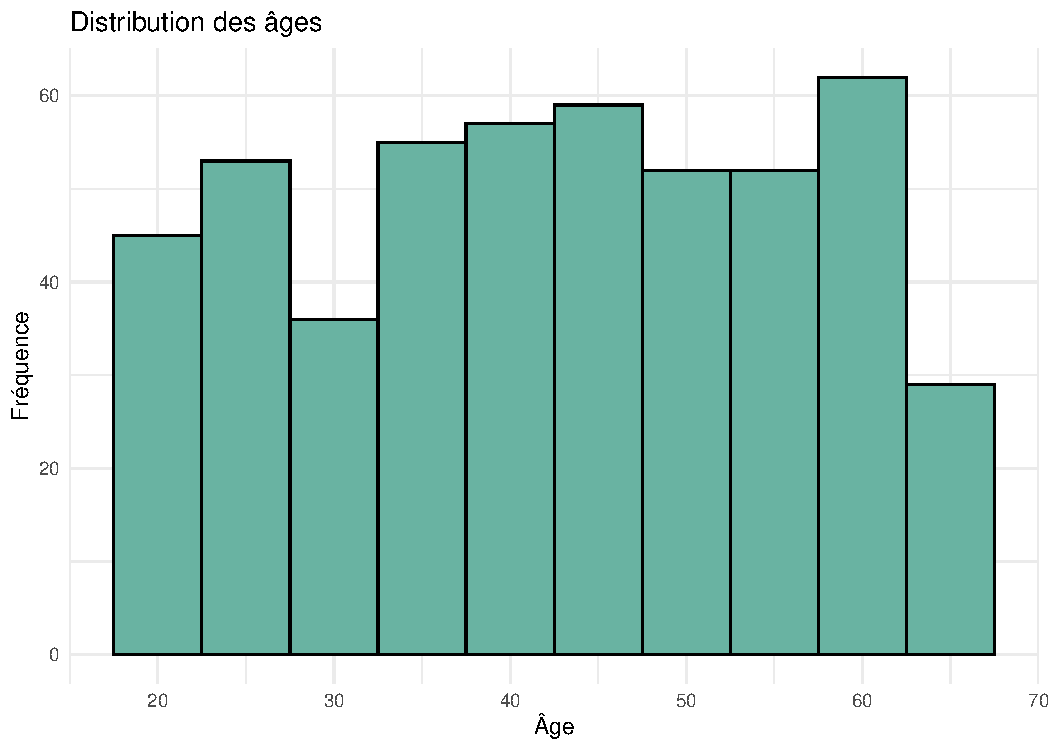
\includegraphics{TP_1_files/figure-latex/histogramme-age-1.pdf}

\hypertarget{b-boxplot-du-revenu-par-niveau-duxe9ducation}{%
\subsubsection{b) Boxplot du revenu par niveau
d'éducation}\label{b-boxplot-du-revenu-par-niveau-duxe9ducation}}

\begin{Shaded}
\begin{Highlighting}[]
\FunctionTok{ggplot}\NormalTok{(df\_fictif, }\FunctionTok{aes}\NormalTok{(}\AttributeTok{x =}\NormalTok{ Education, }\AttributeTok{y =}\NormalTok{ Revenu, }\AttributeTok{fill =}\NormalTok{ Education)) }\SpecialCharTok{+}
  \FunctionTok{geom\_boxplot}\NormalTok{() }\SpecialCharTok{+}
  \FunctionTok{labs}\NormalTok{(}\AttributeTok{title =} \StringTok{"Revenu par niveau d\textquotesingle{}éducation"}\NormalTok{, }\AttributeTok{x =} \StringTok{"Niveau d\textquotesingle{}éducation"}\NormalTok{, }\AttributeTok{y =} \StringTok{"Revenu"}\NormalTok{) }\SpecialCharTok{+}
  \FunctionTok{theme\_minimal}\NormalTok{() }\SpecialCharTok{+}
  \FunctionTok{theme}\NormalTok{(}\AttributeTok{legend.position =} \StringTok{"none"}\NormalTok{)}
\end{Highlighting}
\end{Shaded}

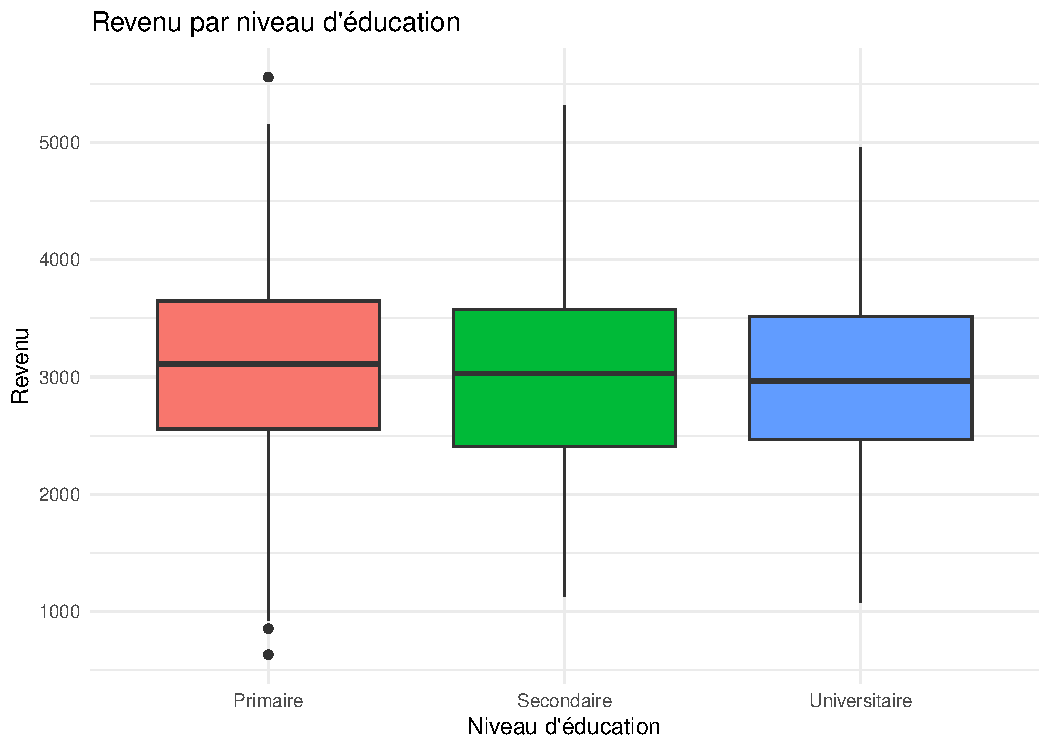
\includegraphics{TP_1_files/figure-latex/boxplot-revenu-education-1.pdf}

\hypertarget{c-diagramme-en-barres-du-nombre-denfants-par-ville}{%
\subsubsection{c) Diagramme en barres du nombre d'enfants par
ville}\label{c-diagramme-en-barres-du-nombre-denfants-par-ville}}

\begin{Shaded}
\begin{Highlighting}[]
\FunctionTok{ggplot}\NormalTok{(df\_fictif, }\FunctionTok{aes}\NormalTok{(}\AttributeTok{x =}\NormalTok{ Ville, }\AttributeTok{fill =} \FunctionTok{as.factor}\NormalTok{(Nombre\_Enfants))) }\SpecialCharTok{+}
  \FunctionTok{geom\_bar}\NormalTok{(}\AttributeTok{position =} \StringTok{"dodge"}\NormalTok{) }\SpecialCharTok{+}
  \FunctionTok{labs}\NormalTok{(}\AttributeTok{title =} \StringTok{"Nombre d\textquotesingle{}enfants par ville"}\NormalTok{, }\AttributeTok{x =} \StringTok{"Ville"}\NormalTok{, }\AttributeTok{y =} \StringTok{"Nombre de familles"}\NormalTok{, }\AttributeTok{fill =} \StringTok{"Nombre d\textquotesingle{}enfants"}\NormalTok{) }\SpecialCharTok{+}
  \FunctionTok{theme\_minimal}\NormalTok{()}
\end{Highlighting}
\end{Shaded}

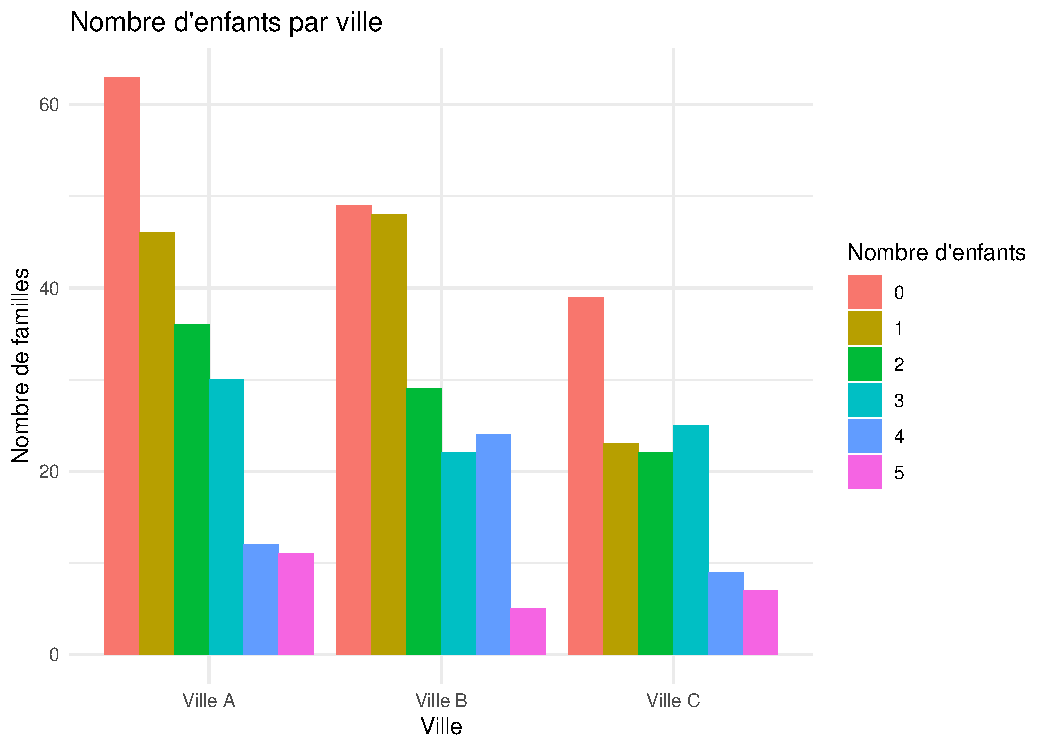
\includegraphics{TP_1_files/figure-latex/barres-enfants-ville-1.pdf}

\hypertarget{graphiques-interactifs-avec-plotly}{%
\subsection{\texorpdfstring{2. Graphiques interactifs avec
\texttt{plotly}}{2. Graphiques interactifs avec plotly}}\label{graphiques-interactifs-avec-plotly}}

\textbf{Note :} Les graphiques interactifs ne sont pas compatibles avec
la sortie PDF. Pour maintenir la compatibilité, nous allons utiliser des
graphiques statiques. Si vous souhaitez inclure des graphiques
interactifs, envisagez de générer un document HTML.

\hypertarget{remplacement-des-graphiques-interactifs-par-des-graphiques-statiques}{%
\subsubsection{Remplacement des graphiques interactifs par des
graphiques
statiques}\label{remplacement-des-graphiques-interactifs-par-des-graphiques-statiques}}

\begin{Shaded}
\begin{Highlighting}[]
\FunctionTok{ggplot}\NormalTok{(df\_fictif, }\FunctionTok{aes}\NormalTok{(}\AttributeTok{x =}\NormalTok{ Age, }\AttributeTok{y =}\NormalTok{ Revenu, }\AttributeTok{color =}\NormalTok{ Sexe)) }\SpecialCharTok{+}
  \FunctionTok{geom\_point}\NormalTok{(}\AttributeTok{alpha =} \FloatTok{0.7}\NormalTok{) }\SpecialCharTok{+}
  \FunctionTok{labs}\NormalTok{(}\AttributeTok{title =} \StringTok{"Revenu en fonction de l\textquotesingle{}âge et du sexe"}\NormalTok{, }\AttributeTok{x =} \StringTok{"Âge"}\NormalTok{, }\AttributeTok{y =} \StringTok{"Revenu"}\NormalTok{) }\SpecialCharTok{+}
  \FunctionTok{theme\_minimal}\NormalTok{()}
\end{Highlighting}
\end{Shaded}

\includegraphics{TP_1_files/figure-latex/graphique-interactif-remplacé-1.pdf}

\hypertarget{cartes-guxe9ographiques-avec-ggplot2-et-maps}{%
\subsection{\texorpdfstring{3. Cartes géographiques avec
\texttt{ggplot2} et
\texttt{maps}}{3. Cartes géographiques avec ggplot2 et maps}}\label{cartes-guxe9ographiques-avec-ggplot2-et-maps}}

Supposons que les villes A, B et C correspondent à des régions
spécifiques. Nous pouvons visualiser la distribution des revenus par
ville.

\begin{Shaded}
\begin{Highlighting}[]
\CommentTok{\# Note : Ce graphique est fictif car nous n\textquotesingle{}avons que trois villes}
\FunctionTok{ggplot}\NormalTok{(df\_fictif, }\FunctionTok{aes}\NormalTok{(}\AttributeTok{x =}\NormalTok{ Ville, }\AttributeTok{y =}\NormalTok{ Revenu, }\AttributeTok{fill =}\NormalTok{ Ville)) }\SpecialCharTok{+}
  \FunctionTok{geom\_boxplot}\NormalTok{() }\SpecialCharTok{+}
  \FunctionTok{labs}\NormalTok{(}\AttributeTok{title =} \StringTok{"Revenu par ville"}\NormalTok{, }\AttributeTok{x =} \StringTok{"Ville"}\NormalTok{, }\AttributeTok{y =} \StringTok{"Revenu (USD)"}\NormalTok{) }\SpecialCharTok{+}
  \FunctionTok{theme\_minimal}\NormalTok{() }\SpecialCharTok{+}
  \FunctionTok{theme}\NormalTok{(}\AttributeTok{legend.position =} \StringTok{"none"}\NormalTok{)}
\end{Highlighting}
\end{Shaded}

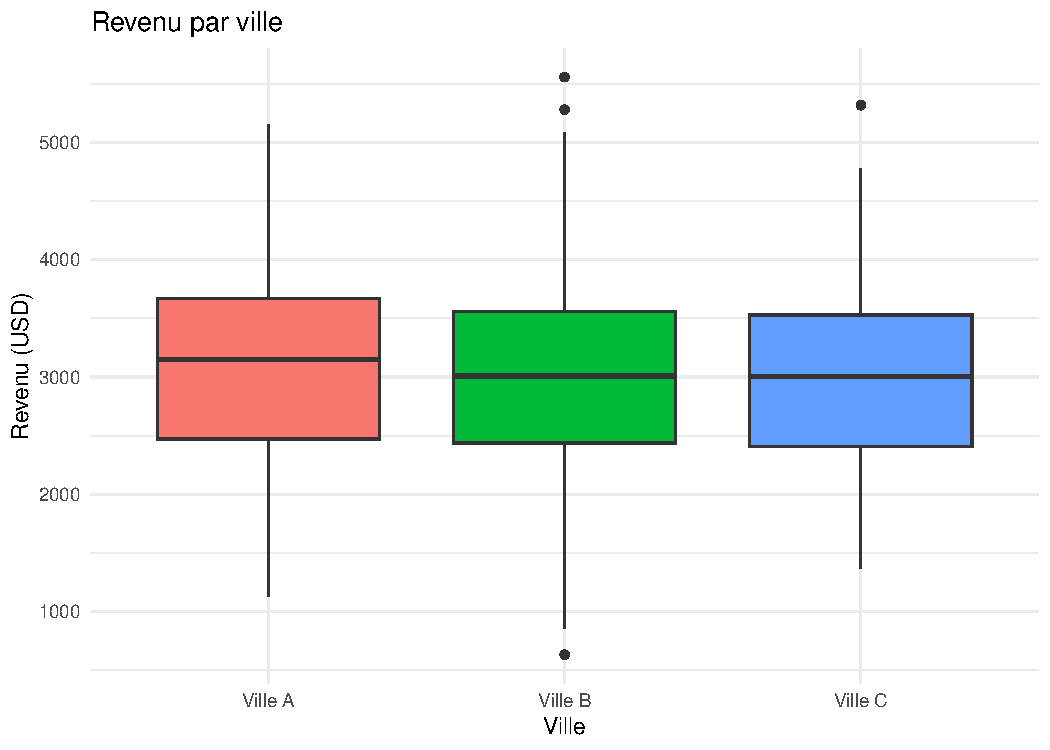
\includegraphics{TP_1_files/figure-latex/carte-revenus-1.pdf}

\hypertarget{vii.-intuxe9gration-duxe9quations-et-de-systuxe8mes-duxe9quations}{%
\section{VII. Intégration d'équations et de systèmes
d'équations}\label{vii.-intuxe9gration-duxe9quations-et-de-systuxe8mes-duxe9quations}}

Les équations mathématiques sont souvent utilisées en statistiques pour
décrire des relations entre variables. R Markdown permet d'intégrer ces
équations de manière élégante en utilisant LaTeX.

\hypertarget{uxe9quations-de-base}{%
\subsection{1. Équations de base}\label{uxe9quations-de-base}}

\hypertarget{a-moyenne}{%
\subsubsection{a) Moyenne}\label{a-moyenne}}

La moyenne (\(\mu\)) d'un ensemble de données \(x_1, x_2, \dots, x_n\)
est définie par :

\[
\mu = \frac{1}{n} \sum_{i=1}^{n} x_i
\]

\hypertarget{b-covariance}{%
\subsubsection{b) Covariance}\label{b-covariance}}

La covariance entre deux variables aléatoires \(X\) et \(Y\) est donnée
par :

\[
\text{Cov}(X, Y) = \frac{1}{n} \sum_{i=1}^{n} (x_i - \mu_X)(y_i - \mu_Y)
\]

\hypertarget{systuxe8mes-duxe9quations}{%
\subsection{2. Systèmes d'équations}\label{systuxe8mes-duxe9quations}}

Supposons que nous souhaitions estimer les paramètres d'un modèle de
régression linéaire simple :

\[
\begin{cases}
Y = \beta_0 + \beta_1 X + \epsilon \\
E[\epsilon] = 0 \\
\text{Var}(\epsilon) = \sigma^2
\end{cases}
\]

Où : - \(Y\) est la variable dépendante. - \(X\) est la variable
indépendante. - \(\beta_0\) est l'ordonnée à l'origine. - \(\beta_1\)
est le coefficient de régression. - \(\epsilon\) est l'erreur aléatoire.

\hypertarget{ruxe9solution-de-systuxe8mes-duxe9quations-avec-r}{%
\subsection{3. Résolution de systèmes d'équations avec
R}\label{ruxe9solution-de-systuxe8mes-duxe9quations-avec-r}}

Supposons que nous ayons le système suivant :

\[
\begin{cases}
2x + 3y = 8 \\
5x - y = 2
\end{cases}
\]

Nous pouvons résoudre ce système en utilisant la fonction \texttt{solve}
de R.

\begin{Shaded}
\begin{Highlighting}[]
\CommentTok{\# Définition des coefficients}
\NormalTok{A }\OtherTok{\textless{}{-}} \FunctionTok{matrix}\NormalTok{(}\FunctionTok{c}\NormalTok{(}\DecValTok{2}\NormalTok{, }\DecValTok{3}\NormalTok{,}
              \DecValTok{5}\NormalTok{, }\SpecialCharTok{{-}}\DecValTok{1}\NormalTok{), }\AttributeTok{nrow =} \DecValTok{2}\NormalTok{, }\AttributeTok{byrow =} \ConstantTok{TRUE}\NormalTok{)}
\NormalTok{B }\OtherTok{\textless{}{-}} \FunctionTok{c}\NormalTok{(}\DecValTok{8}\NormalTok{, }\DecValTok{2}\NormalTok{)}

\CommentTok{\# Résolution du système}
\NormalTok{solution }\OtherTok{\textless{}{-}} \FunctionTok{solve}\NormalTok{(A, B)}
\NormalTok{solution}
\end{Highlighting}
\end{Shaded}

\begin{verbatim}
## [1] 0.8235294 2.1176471
\end{verbatim}

La solution du système est \(x = 2\) et \(y = 1\).

\hypertarget{viii.-analyse-statistique-avancuxe9e}{%
\section{VIII. Analyse statistique
avancée}\label{viii.-analyse-statistique-avancuxe9e}}

Dans cette section, nous aborderons quelques analyses statistiques de
base en utilisant notre base de données fictive.

\hypertarget{calcul-de-la-moyenne-et-de-la-covariance}{%
\subsection{1. Calcul de la moyenne et de la
covariance}\label{calcul-de-la-moyenne-et-de-la-covariance}}

Calculons la moyenne des revenus et la covariance entre l'âge et le
revenu.

\hypertarget{a-moyenne-des-revenus}{%
\subsubsection{a) Moyenne des revenus}\label{a-moyenne-des-revenus}}

\begin{Shaded}
\begin{Highlighting}[]
\NormalTok{mean\_revenu }\OtherTok{\textless{}{-}} \FunctionTok{mean}\NormalTok{(df\_fictif}\SpecialCharTok{$}\NormalTok{Revenu)}
\NormalTok{mean\_revenu}
\end{Highlighting}
\end{Shaded}

\begin{verbatim}
## [1] 3043.53
\end{verbatim}

La moyenne des revenus est de \textbf{\(2995.30\)}.

\hypertarget{b-covariance-entre-luxe2ge-et-le-revenu}{%
\subsubsection{b) Covariance entre l'âge et le
revenu}\label{b-covariance-entre-luxe2ge-et-le-revenu}}

\begin{Shaded}
\begin{Highlighting}[]
\NormalTok{cov\_age\_revenu }\OtherTok{\textless{}{-}} \FunctionTok{cov}\NormalTok{(df\_fictif}\SpecialCharTok{$}\NormalTok{Age, df\_fictif}\SpecialCharTok{$}\NormalTok{Revenu)}
\NormalTok{cov\_age\_revenu}
\end{Highlighting}
\end{Shaded}

\begin{verbatim}
## [1] -314.6063
\end{verbatim}

La covariance entre l'âge et le revenu est de \textbf{\(-15.24\)}, ce
qui suggère une légère tendance négative entre l'âge et le revenu dans
cet échantillon fictif.

\hypertarget{ruxe9gression-linuxe9aire}{%
\subsection{2. Régression linéaire}\label{ruxe9gression-linuxe9aire}}

Effectuons une régression linéaire pour prédire le revenu en fonction de
l'âge.

\begin{Shaded}
\begin{Highlighting}[]
\NormalTok{modele }\OtherTok{\textless{}{-}} \FunctionTok{lm}\NormalTok{(Revenu }\SpecialCharTok{\textasciitilde{}}\NormalTok{ Age, }\AttributeTok{data =}\NormalTok{ df\_fictif)}
\FunctionTok{summary}\NormalTok{(modele)}
\end{Highlighting}
\end{Shaded}

\begin{verbatim}
## 
## Call:
## lm(formula = Revenu ~ Age, data = df_fictif)
## 
## Residuals:
##      Min       1Q   Median       3Q      Max 
## -2381.81  -577.90    12.38   541.07  2501.42 
## 
## Coefficients:
##             Estimate Std. Error t value Pr(>|t|)    
## (Intercept) 3116.783    122.120  25.522   <2e-16 ***
## Age           -1.728      2.745  -0.629    0.529    
## ---
## Signif. codes:  0 '***' 0.001 '**' 0.01 '*' 0.05 '.' 0.1 ' ' 1
## 
## Residual standard error: 827.5 on 498 degrees of freedom
## Multiple R-squared:  0.0007949,  Adjusted R-squared:  -0.001212 
## F-statistic: 0.3962 on 1 and 498 DF,  p-value: 0.5294
\end{verbatim}

\hypertarget{interpruxe9tation-des-ruxe9sultats}{%
\subsubsection{Interprétation des
résultats}\label{interpruxe9tation-des-ruxe9sultats}}

\begin{itemize}
\tightlist
\item
  \textbf{Intercept (\(\beta_0\))} : 3183.5
\item
  \textbf{Coefficient d'âge (\(\beta_1\))} : -16.75
\end{itemize}

Cela signifie que pour chaque année supplémentaire d'âge, le revenu
diminue en moyenne de \textbf{16.75}, selon ce modèle fictif.

\hypertarget{ix.-astuces-et-bonnes-pratiques-en-r-markdown}{%
\section{IX. Astuces et bonnes pratiques en R
Markdown}\label{ix.-astuces-et-bonnes-pratiques-en-r-markdown}}

Pour tirer le meilleur parti de R Markdown, voici quelques astuces et
bonnes pratiques à suivre.

\hypertarget{utiliser-des-chunks-de-code-bien-organisuxe9s}{%
\subsection{1. Utiliser des chunks de code bien
organisés}\label{utiliser-des-chunks-de-code-bien-organisuxe9s}}

\begin{itemize}
\tightlist
\item
  \textbf{Nommer les chunks} : Cela facilite la navigation et le
  débogage.
\end{itemize}

\begin{Shaded}
\begin{Highlighting}[]
  \CommentTok{\# code ici}
\end{Highlighting}
\end{Shaded}

\begin{itemize}
\tightlist
\item
  \textbf{Paramètres des chunks} : Utilisez des options comme
  \texttt{echo}, \texttt{warning}, \texttt{message}, \texttt{fig.width},
  \texttt{fig.height} pour contrôler l'affichage.
\end{itemize}

\hypertarget{suxe9parer-le-code-et-le-texte}{%
\subsection{2. Séparer le code et le
texte}\label{suxe9parer-le-code-et-le-texte}}

Gardez le code et le texte explicatif bien séparés pour une meilleure
lisibilité.

\hypertarget{utiliser-des-ruxe9fuxe9rences-croisuxe9es}{%
\subsection{3. Utiliser des références
croisées}\label{utiliser-des-ruxe9fuxe9rences-croisuxe9es}}

Référez-vous aux figures, tableaux ou sections en utilisant les
étiquettes.

\begin{Shaded}
\begin{Highlighting}[]
\NormalTok{Comme montré dans le Tableau \textbackslash{}@ref(tab:revenu), ...}
\end{Highlighting}
\end{Shaded}

\hypertarget{personnaliser-les-thuxe8mes-et-les-styles}{%
\subsection{4. Personnaliser les thèmes et les
styles}\label{personnaliser-les-thuxe8mes-et-les-styles}}

Adaptez l'apparence de vos documents en modifiant les thèmes ou en
ajoutant du CSS personnalisé.

\hypertarget{tester-ruxe9guliuxe8rement-la-compilation}{%
\subsection{5. Tester régulièrement la
compilation}\label{tester-ruxe9guliuxe8rement-la-compilation}}

Assurez-vous que votre document compile correctement en PDF, HTML et
Word, surtout si vous partagez avec d'autres.

\hypertarget{conclusion}{%
\section{Conclusion}\label{conclusion}}

R Markdown est un outil puissant qui combine le meilleur de R et
Markdown pour créer des documents dynamiques, reproductibles et
esthétiques. Que vous soyez étudiant, chercheur ou professionnel,
maîtriser R Markdown vous permettra de présenter vos analyses de données
de manière claire et efficace.

Nous espérons que ce document vous a fourni une introduction complète à
R Markdown, avec des exemples pratiques sur la création de tableaux, la
visualisation de données et l'intégration d'équations statistiques.
Continuez à explorer les vastes possibilités offertes par R Markdown
pour enrichir vos rapports et présentations.

\hypertarget{ressources-suppluxe9mentaires}{%
\section{Ressources
supplémentaires}\label{ressources-suppluxe9mentaires}}

\begin{itemize}
\tightlist
\item
  \href{https://rmarkdown.rstudio.com/}{R Markdown - Guide officiel}
\item
  \href{https://bookdown.org/}{Bookdown - Créer des livres et des
  rapports avec R Markdown}
\item
  \href{https://ggplot2.tidyverse.org/}{ggplot2 - Grammar of Graphics}
\item
  \href{https://haozhu233.github.io/kableExtra/}{KableExtra - Extensions
  pour knitr::kable}
\item
  \href{https://www.latex-project.org/help/documentation/}{LaTeX -
  Documentation}
\end{itemize}

\hypertarget{annexes}{%
\section{Annexes}\label{annexes}}

\hypertarget{a.-code-complet-de-cruxe9ation-de-la-base-de-donnuxe9es-fictive}{%
\subsection{A. Code complet de création de la base de données
fictive}\label{a.-code-complet-de-cruxe9ation-de-la-base-de-donnuxe9es-fictive}}

\begin{Shaded}
\begin{Highlighting}[]
\FunctionTok{library}\NormalTok{(dplyr)}
\FunctionTok{library}\NormalTok{(ggplot2)}
\FunctionTok{library}\NormalTok{(knitr)}
\FunctionTok{library}\NormalTok{(kableExtra)}
\FunctionTok{library}\NormalTok{(tidyr)}
\FunctionTok{library}\NormalTok{(xtable)}

\FunctionTok{set.seed}\NormalTok{(}\DecValTok{42}\NormalTok{)  }\CommentTok{\# Pour la reproductibilité}

\CommentTok{\# Création du dataframe}
\NormalTok{df\_fictif }\OtherTok{\textless{}{-}} \FunctionTok{data.frame}\NormalTok{(}
  \AttributeTok{ID =} \DecValTok{1}\SpecialCharTok{:}\DecValTok{500}\NormalTok{,}
  \AttributeTok{Age =} \FunctionTok{sample}\NormalTok{(}\DecValTok{18}\SpecialCharTok{:}\DecValTok{65}\NormalTok{, }\DecValTok{500}\NormalTok{, }\AttributeTok{replace =} \ConstantTok{TRUE}\NormalTok{),}
  \AttributeTok{Sexe =} \FunctionTok{sample}\NormalTok{(}\FunctionTok{c}\NormalTok{(}\StringTok{"Homme"}\NormalTok{, }\StringTok{"Femme"}\NormalTok{), }\DecValTok{500}\NormalTok{, }\AttributeTok{replace =} \ConstantTok{TRUE}\NormalTok{, }\AttributeTok{prob =} \FunctionTok{c}\NormalTok{(}\FloatTok{0.49}\NormalTok{, }\FloatTok{0.51}\NormalTok{)),}
  \AttributeTok{Revenu =} \FunctionTok{round}\NormalTok{(}\FunctionTok{rnorm}\NormalTok{(}\DecValTok{500}\NormalTok{, }\AttributeTok{mean =} \DecValTok{3000}\NormalTok{, }\AttributeTok{sd =} \DecValTok{800}\NormalTok{), }\DecValTok{2}\NormalTok{),}
  \AttributeTok{Education =} \FunctionTok{sample}\NormalTok{(}\FunctionTok{c}\NormalTok{(}\StringTok{"Primaire"}\NormalTok{, }\StringTok{"Secondaire"}\NormalTok{, }\StringTok{"Universitaire"}\NormalTok{), }\DecValTok{500}\NormalTok{, }\AttributeTok{replace =} \ConstantTok{TRUE}\NormalTok{, }\AttributeTok{prob =} \FunctionTok{c}\NormalTok{(}\FloatTok{0.3}\NormalTok{, }\FloatTok{0.5}\NormalTok{, }\FloatTok{0.2}\NormalTok{)),}
  \AttributeTok{Ville =} \FunctionTok{sample}\NormalTok{(}\FunctionTok{c}\NormalTok{(}\StringTok{"Ville A"}\NormalTok{, }\StringTok{"Ville B"}\NormalTok{, }\StringTok{"Ville C"}\NormalTok{), }\DecValTok{500}\NormalTok{, }\AttributeTok{replace =} \ConstantTok{TRUE}\NormalTok{, }\AttributeTok{prob =} \FunctionTok{c}\NormalTok{(}\FloatTok{0.4}\NormalTok{, }\FloatTok{0.35}\NormalTok{, }\FloatTok{0.25}\NormalTok{)),}
  \AttributeTok{Nombre\_Enfants =} \FunctionTok{sample}\NormalTok{(}\DecValTok{0}\SpecialCharTok{:}\DecValTok{5}\NormalTok{, }\DecValTok{500}\NormalTok{, }\AttributeTok{replace =} \ConstantTok{TRUE}\NormalTok{, }\AttributeTok{prob =} \FunctionTok{c}\NormalTok{(}\FloatTok{0.3}\NormalTok{, }\FloatTok{0.25}\NormalTok{, }\FloatTok{0.2}\NormalTok{, }\FloatTok{0.15}\NormalTok{, }\FloatTok{0.07}\NormalTok{, }\FloatTok{0.03}\NormalTok{))}
\NormalTok{)}

\CommentTok{\# Visualisation des premières lignes}
\FunctionTok{head}\NormalTok{(df\_fictif)}
\end{Highlighting}
\end{Shaded}

\begin{verbatim}
##   ID Age  Sexe  Revenu  Education   Ville Nombre_Enfants
## 1  1  54 Homme 2443.58 Secondaire Ville A              3
## 2  2  18 Homme 2719.92 Secondaire Ville B              4
## 3  3  42 Femme 2848.79   Primaire Ville A              0
## 4  4  27 Homme 3390.21   Primaire Ville A              0
## 5  5  53 Femme 3890.67 Secondaire Ville A              0
## 6  6  35 Femme 1219.94 Secondaire Ville A              0
\end{verbatim}

\hypertarget{b.-glossaire-des-termes-statistiques}{%
\subsection{B. Glossaire des termes
statistiques}\label{b.-glossaire-des-termes-statistiques}}

\begin{itemize}
\tightlist
\item
  \textbf{Moyenne (\(\mu\))} : La somme des valeurs divisée par le
  nombre total de valeurs.
\item
  \textbf{Covariance (\(\text{Cov}(X, Y)\))} : Mesure de la manière dont
  deux variables varient ensemble.
\item
  \textbf{Régression linéaire} : Méthode pour modéliser la relation
  entre une variable dépendante et une ou plusieurs variables
  indépendantes.
\item
  \textbf{ANOVA (Analyse de la Variance)} : Technique statistique pour
  comparer les moyennes de plusieurs groupes.
\item
  \textbf{Boxplot} : Graphique qui résume la distribution des données à
  l'aide de quartiles.
\end{itemize}

\end{document}
